%!TEX root = ../thesis.tex
%*******************************************************************************
%******************************   Fourth Chapter   ***************************
%*******************************************************************************
\chapter{Improving \ont{} sequencing accuracy for \mtb{}}
\label{chap:tubby}
%%%%%%%%%%%%%%%%%%%%%%%%%%%%%%%%%%%%%%%%%%%%%%%%%%%%%%%%%%%%%%%%%%%%%%%%%%%%%%%%%

\setcounter{section}{-1}
\section{Publication and collaboration acknowledgements}
\label{sec:ch4-acknowledge}

%%%%%%%%%%%%%%%%%%%%%%%%%%%%%%%%%%%%%%%%%%%%%%%%%%%%%%%%%%%%%%%%%%%%%%%%%%%%%%%%%
\section{Introduction}

Taxon-specific \ont{} basecalling models have been shown to provide increased read and consensus accuracy(CITE).
It has previously been shown(CITE) that a taxon-specific basecalling model can improve both the read-level and consensus accuracy of \ont{} sequencing reads. While this was shown for *Klebsiella pneumoniae*, it remains to be seen if this approach generalises to other species.

%%%%%%%%%%%%%%%%%%%%%%%%%%%%%%%%%%%%%%%%%%%%%%%%%%%%%%%%%%%%%%%%%%%%%%%%%%%%%%%%%
\section{Dataset}
\label{sec:tubby-data}

 Perhaps the most important aspect of training a basecalling model is providing a "truth" for the data. In the context of training a \ont{} basecalling model, truth data refers to high-quality genome assemblies for the training samples. The \ont{} basecaller, \guppy{}, uses neural networks to convert the raw electrical signal into a DNA sequence. In order to train the network in how to make this inference it is necessary to label the raw signal with its corresponding "truth" sequence. Such datasets are difficult to find for certain species. However, the dataset we have collected for the work \autoref{chap:clustering} and \autoref{chap:dst} is perfectly suited. It contains samples with Illumina, PacBio, and \ont{} sequencing data from the exact same DNA extraction, ensuring any discrepancies between the \ont{} data and the truth are technology differences, and not \textit{in vitro} evolution. 

For the training and validation of our \mtb{}-specific model, we use the eight samples we generated high-quality assemblies from PacBio data in \autoref{sec:asm_results} (see \autoref{app:asm} for full methods). We use the PacBio assemblies produced by \flye{} and polished with Illumina by Pilon - not correcting for SNPs. By using the Illumina-polished PacBio assemblies for each sample we ensure no \ont{} biases are present in the truth genomes that the new model is being trained from.

In addition to the eight training and validation samples, we evaluate on a \ont{} sequencing run of the \textit{Mycobacterium bovis} strain used in the Bacille Calmette-Guérin (BCG) vaccine. This strain (AF2122/97) is an attenuated \textit{M. bovis} bacillus \cite{luca2013} with a well-characterised reference genome (accession LT708304.1) \cite{Malone2017}. As the genome similarity between \textit{M. bovis} and \mtb{} is 99.95\% \cite{Kanipe2020}, this BCG strain acts as a great test for the model's ability to call both a sample not from the training set and not from the exact species, but a very closely related one.

\todo[inline]{add BCG sequencing methods}
%  I have emailed Sophie requesting these methods

%%%%%%%%%%%%%%%%%%%%%%%%%%%%%%%%%%%%%%%%%%%%%%%%%%%%%%%%%%%%%%%%%%%%%%%%%%%%%%%%%
\section{Training an \mtb{}-specific \ont{} basecalling model}

In order to be train a basecalling model for use with \guppy{}, there are a number of preparation steps required. For many of these preparation steps, we use the open-source software, Taiyaki, developed by Oxford Nanopore Technologies (ONT) to train their RNA and DNA model for \guppy{} (\url{https://github.com/nanoporetech/taiyaki}).

We trained an \mtb{}-specific basecalling model - named \tubby{} - for use with three different versions of \guppy{}: 3.4.5, 3.6.0, and 4.4.0. The preparation, training, and evaluation steps are the same for each model, with the only difference being the version of \guppy{} used to basecall the initial data, and the pretrained models used to begin training from.

\subsubsection{Preparation}

In the first stage of preparing the data for training, we basecall and demultiplex the data with the relevant version of \guppy{} using the default high-accuracy model configurations (HAC). Next, we align the basecalled reads for each sample to their truth assembly (\autoref{sec:tubby-data}) with \vrb{minimap2} \cite{li2018}, discarding unmapped and secondary alignments.

The sequence for each aligned read is then replaced with the reference sequence it aligns to - in the same orientation - using \taiyaki{}. Any read with less than 50\%  of its sequence aligned is discarded in this process. The resulting FASTA file from this step acts as a way of mapping a read identifier to its truth sequence during training and contained 1,309,759 read-references.

The recommended number of reads for \taiyaki{} model-training is in the range of tens-of-thousands or low hundreds-of-thousands if read lengths are greater than 1000bp or less than 500bp, respectively. As our read-reference file has many more sequences than is required, we randomly sub-sampled the FASTA file into two chunks with 20\% (261,950) for training and the remainder (1,047,807) to be used for validation of the final model. Using the list of read identifiers in these two subsets, we extract the raw (fast5) data for each read into separate training and evaluation batches. 

Next, we use \taiyaki{} to trim 200 and 100 raw signal events from the start and end, respectively, of each training read. This trimming essentially serves to remove adapter and barcodes signals. \taiyaki{} is then used to align the raw signal for a read to its sequence in the read-reference file. This mapping is a vital preparation step that creates a signal-to-sequence file indicating what nucleotides are associated with a given collection of the raw signals and vice versa.

\begin{figure}
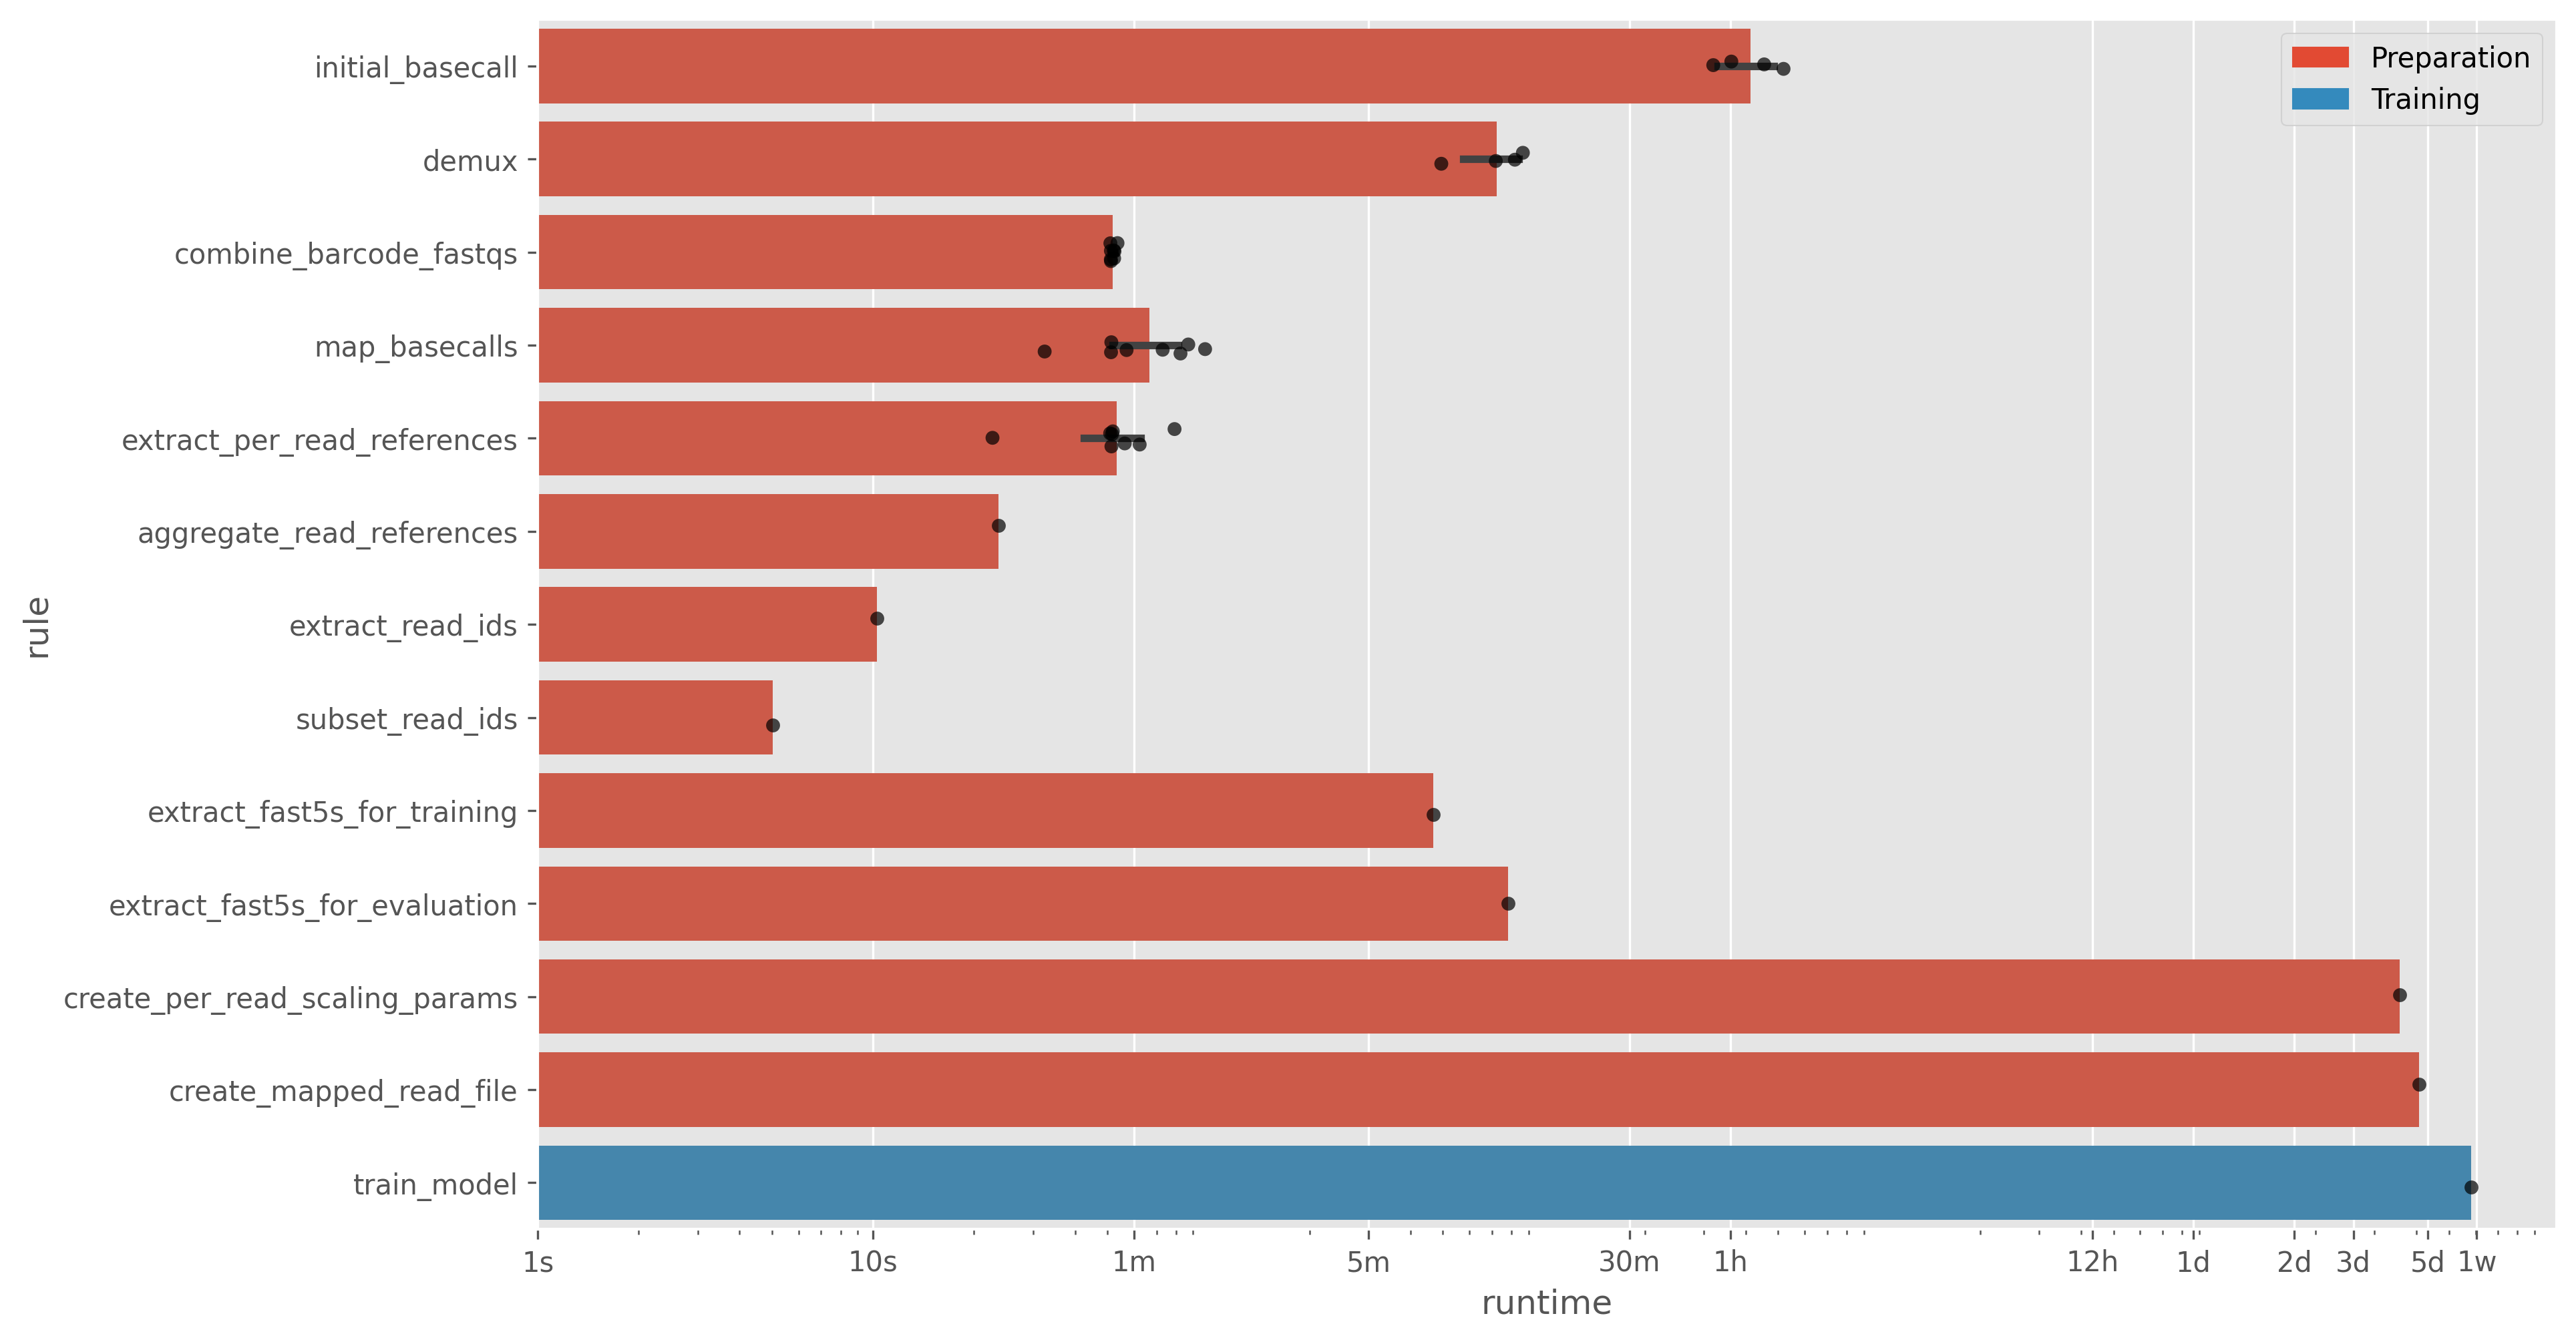
\includegraphics[width=0.9\textwidth]{Chapter4/Figs/prep_runtime.png}
\centering
\caption{Runtimes (x-axis) of the different stages (rules; y-axis) of preparing data for basecall model training. Each individual run is represented with a black point and rules that have multiple runs have black 95\% confidence interval bars. s=seconds; m=minutes; h=hours; d=days.}
\label{fig:prep_runtime}
\end{figure}

\autoref{fig:prep_runtime} shows the runtime of each step in the preparation phase of training. The two longest stages, trimming the raw signal (\vrb{create\_per\_read\_scaling\_params}) and mapping the raw signal to read-references (\vrb{create\_mapped\_read\_file}), took 4.1 and 4.7 days respectively. In total, the full preparation pipeline ran in 8.9 days. 

\subsubsection{Training}

The signal-to-sequencing mapping file produced from the preparation pipeline is the data file used for model training. In addition, we provide an initial model file from which training begins; the mLstm flipflop model distributed with \taiyaki{}.

We train the model using \taiyaki{}'s \vrb{train\_flipflop.py} script with the following parameters: a base layer size of 256; a model stride of 2; a window length over the data of 19; a minimum and maximum length of random training data chunks of 2000 and 4000, respectively; and a maximum learning rate of $0.002\sqrt{g}$, where $g$ is the number of GPUs used for training. The training took 162 hours (6.75 days) to complete on 2 GPUs and had a peak memory usage of 57GB. 

The final output from training the model is a checkpoint file, which we then convert to a \guppy{}-compatible JSON configuration file using \taiyaki{}.

%%%%%%%%%%%%%%%%%%%%%%%%%%%%%%%%%%%%%%%%%%%%%%%%%%%%%%%%%%%%%%%%%%%%%%%%%%%%%%%%%
\section{Evaluating a custom \ont{} basecalling model}

The model-training process produces a JSON file that can be used as a model configuration to basecall \ont{} reads using \guppy{}. The first step in evaluating whether our \mtb{}-specific model, \tubby{}, provides improved accuracy compared to \guppy{}'s default model is to basecall the validation reads that were set aside prior to training. These validation reads provide an unbiased dataset to evaluate on as they were not involved in the training process. 

Although the validation data was not used for training, they are from from the same data source (sample). Therefore, we additionally assess both models on an independent BCG dataset (\autoref{sec:tubby-data}). This BCG sample was not sequenced in the same experiment as the training and validation samples. Additionally, it is a different species (\textit{M. bovis}), but still part of the same genus and the \mtb{} complex (MTBC). As such, it serves as a test of each model's generalisation capabilities. 

We evaluate the read- and consensus-level accuracy of reads produced by \guppy{} and \tubby{} and assess the types of errors made by each. 

% =====
\subsection{Read-level performance}
\label{sec:tubby-read}

The first evaluation metric, read BLAST identity, determines the read-level accuracy produced by the basecalling model. We align the basecalled reads to their respective truth assembly with \vrb{minimap2}, discarding secondary alignments (but keeping unmapped reads). From the resulting pairwise alignment (PAF) file we calculate the BLAST identity as, for each mapping, the number of matching bases divided by the length of the alignment. 

In addition to read BLAST identity, we also assess the relative read lengths produced by each basecalling model. We define relative read length as the length of the aligned part of the read, divided by the total length of the read. The purpose of this metric is to see whether there is a bias towards insertions (greater than 1.0) or deletions (less than 1.0). 

\subsubsection{Validation data}

\autoref{fig:eval-read-blast} shows the distribution of read BLAST identity values for each \guppy{} version and associated \tubby{} model. For all versions, \tubby{} has the highest read BLAST identity values - i.e., distribution of values is tighter, and the mode is further to the right. Interestingly, the best performing version for both models was 3.6.0, with a median BLAST identity of 95.54\% and 94.13\% for \tubby{} and \guppy{} respectively. \autoref{tab:read-blast} describes the summary statistics of the read BLAST identity distributions.

While version 3.6.0 has the highest median values for both models, it is important not to rely on this alone. For instance, version 4.4.0 has the highest minimum value for both models, and the highest mode (\tubby{} version 3.6.0 and 4.4.0 have the same mode). However, the percentiles are highest for version 3.6.0.

\begin{figure}
     \centering
     \begin{subfigure}[b]{0.9\textwidth}
        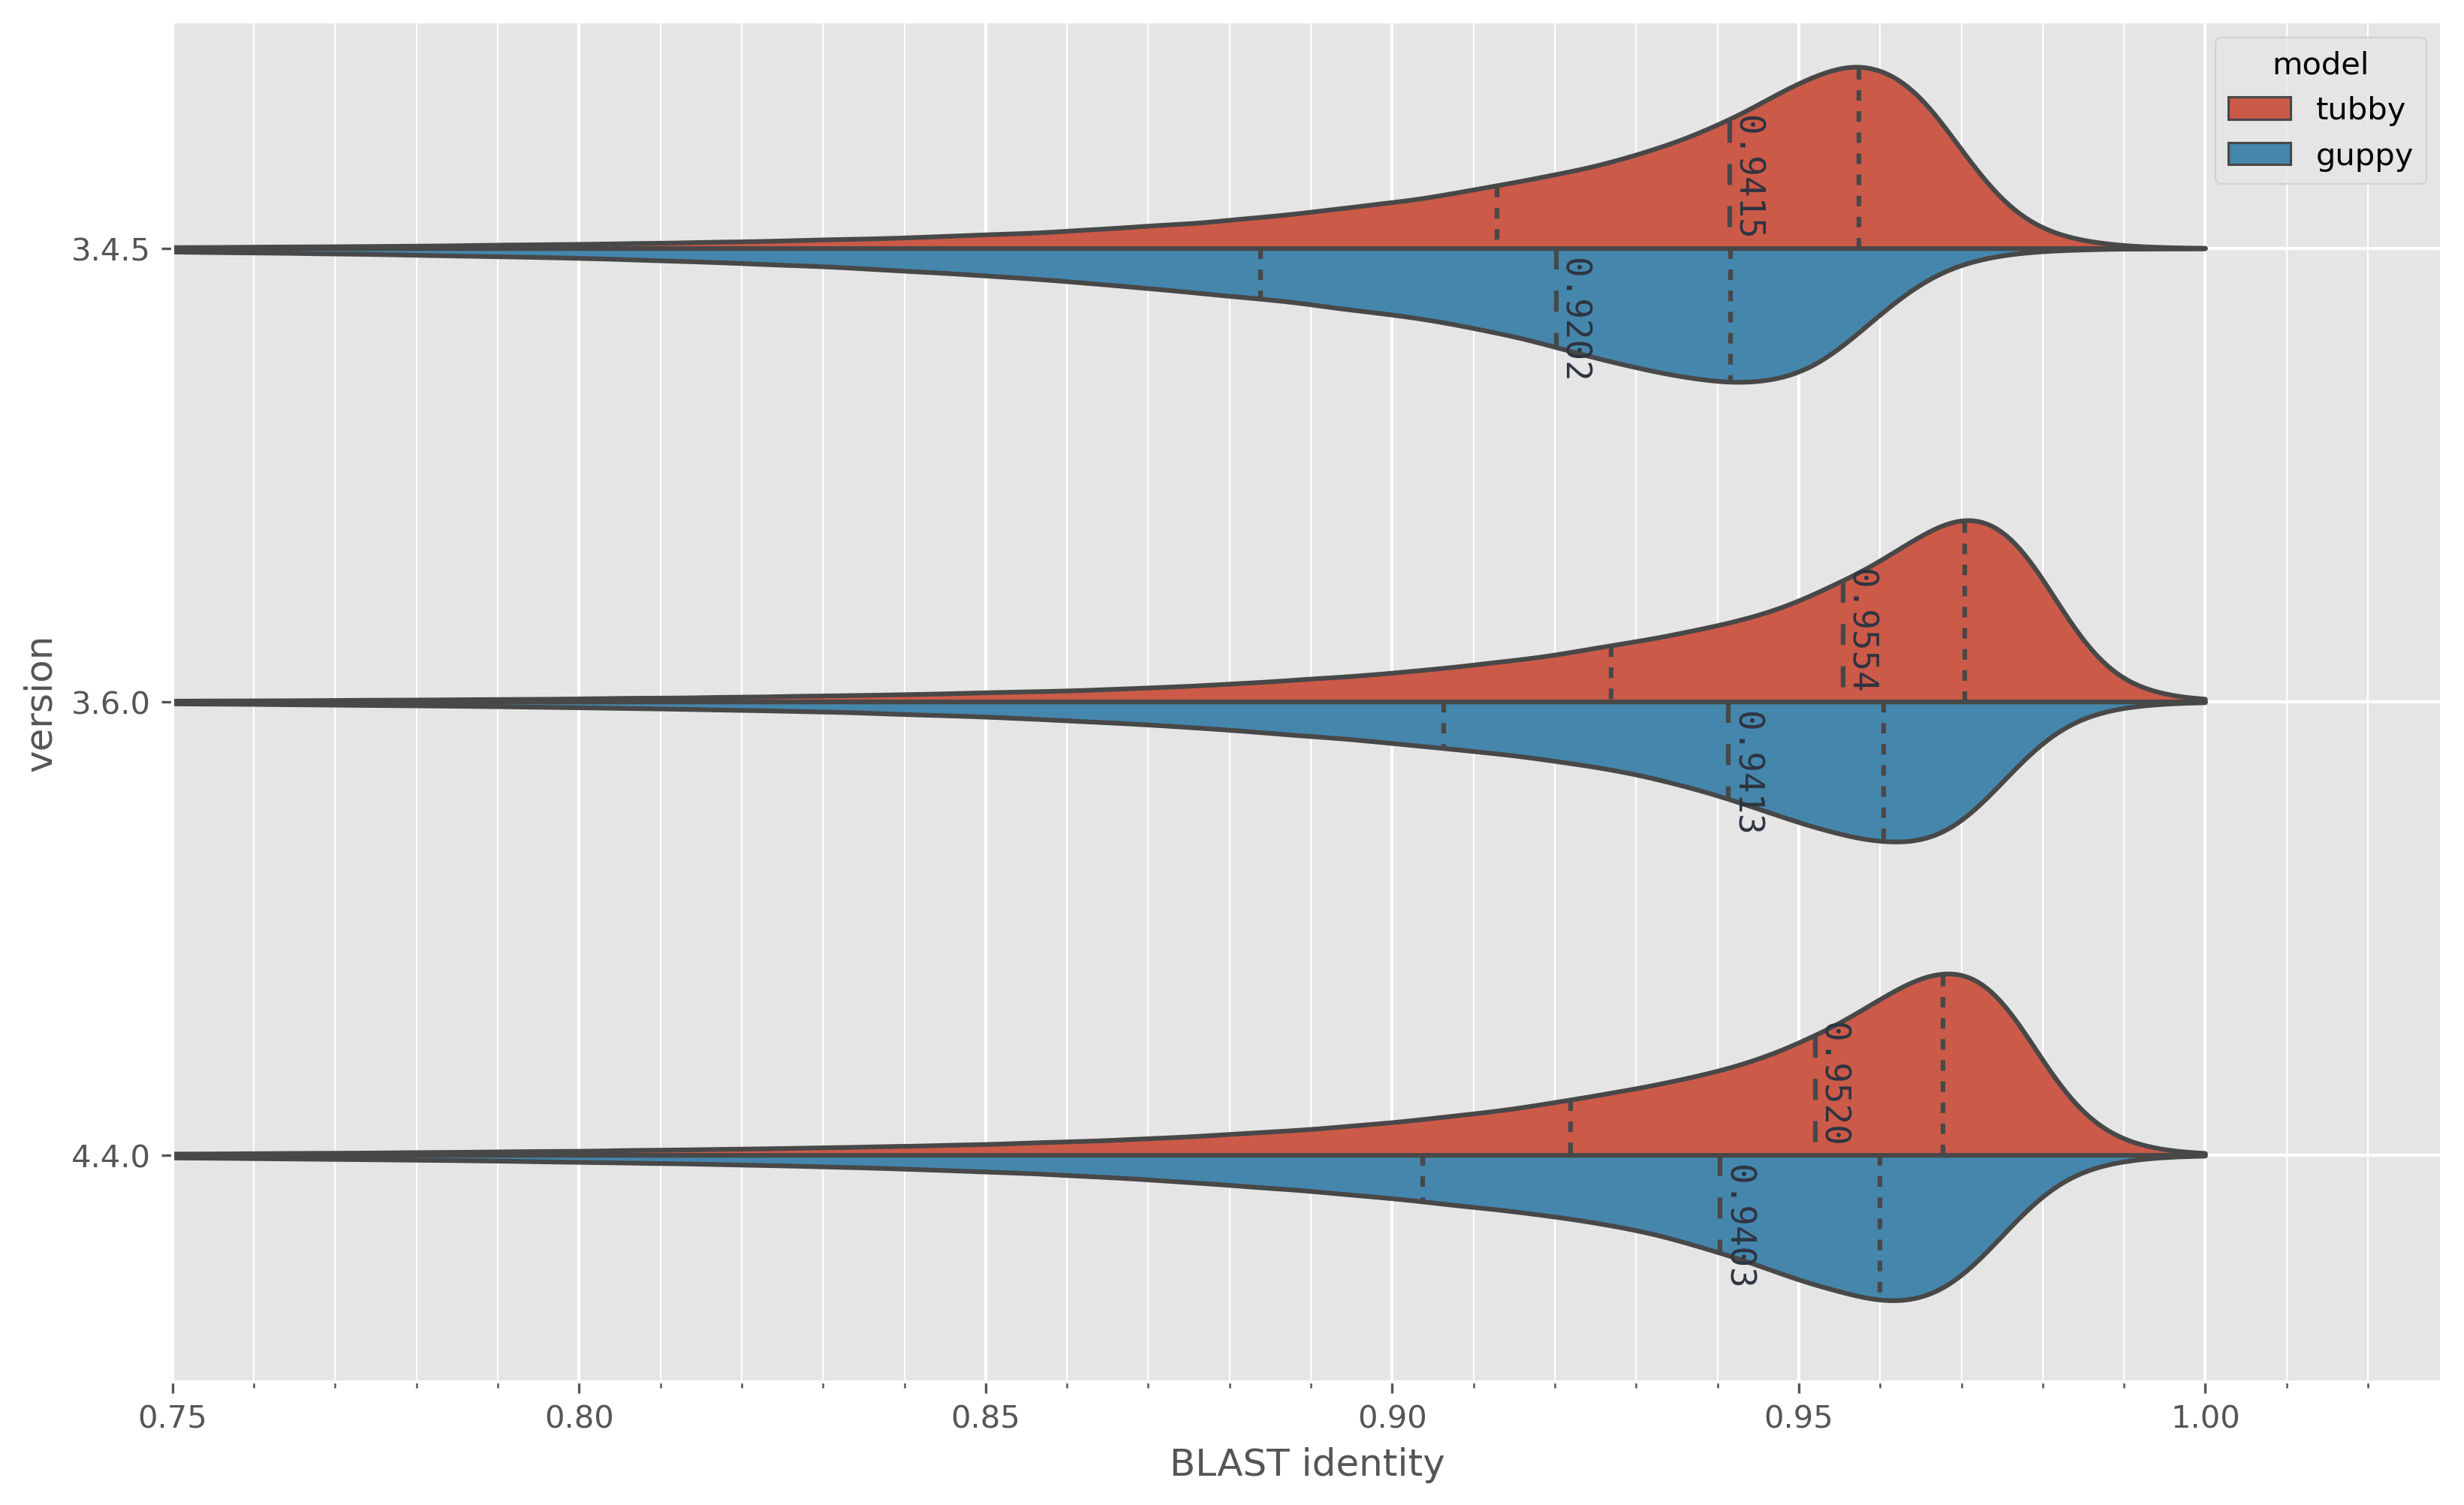
\includegraphics[width=1\linewidth]{Chapter4/Figs/read_blast_identity.png}
        \centering
        \caption{Validation data}
        \label{fig:eval-read-blast}
     \end{subfigure}
     \hfill
     \begin{subfigure}[b]{0.9\textwidth}
         \centering
        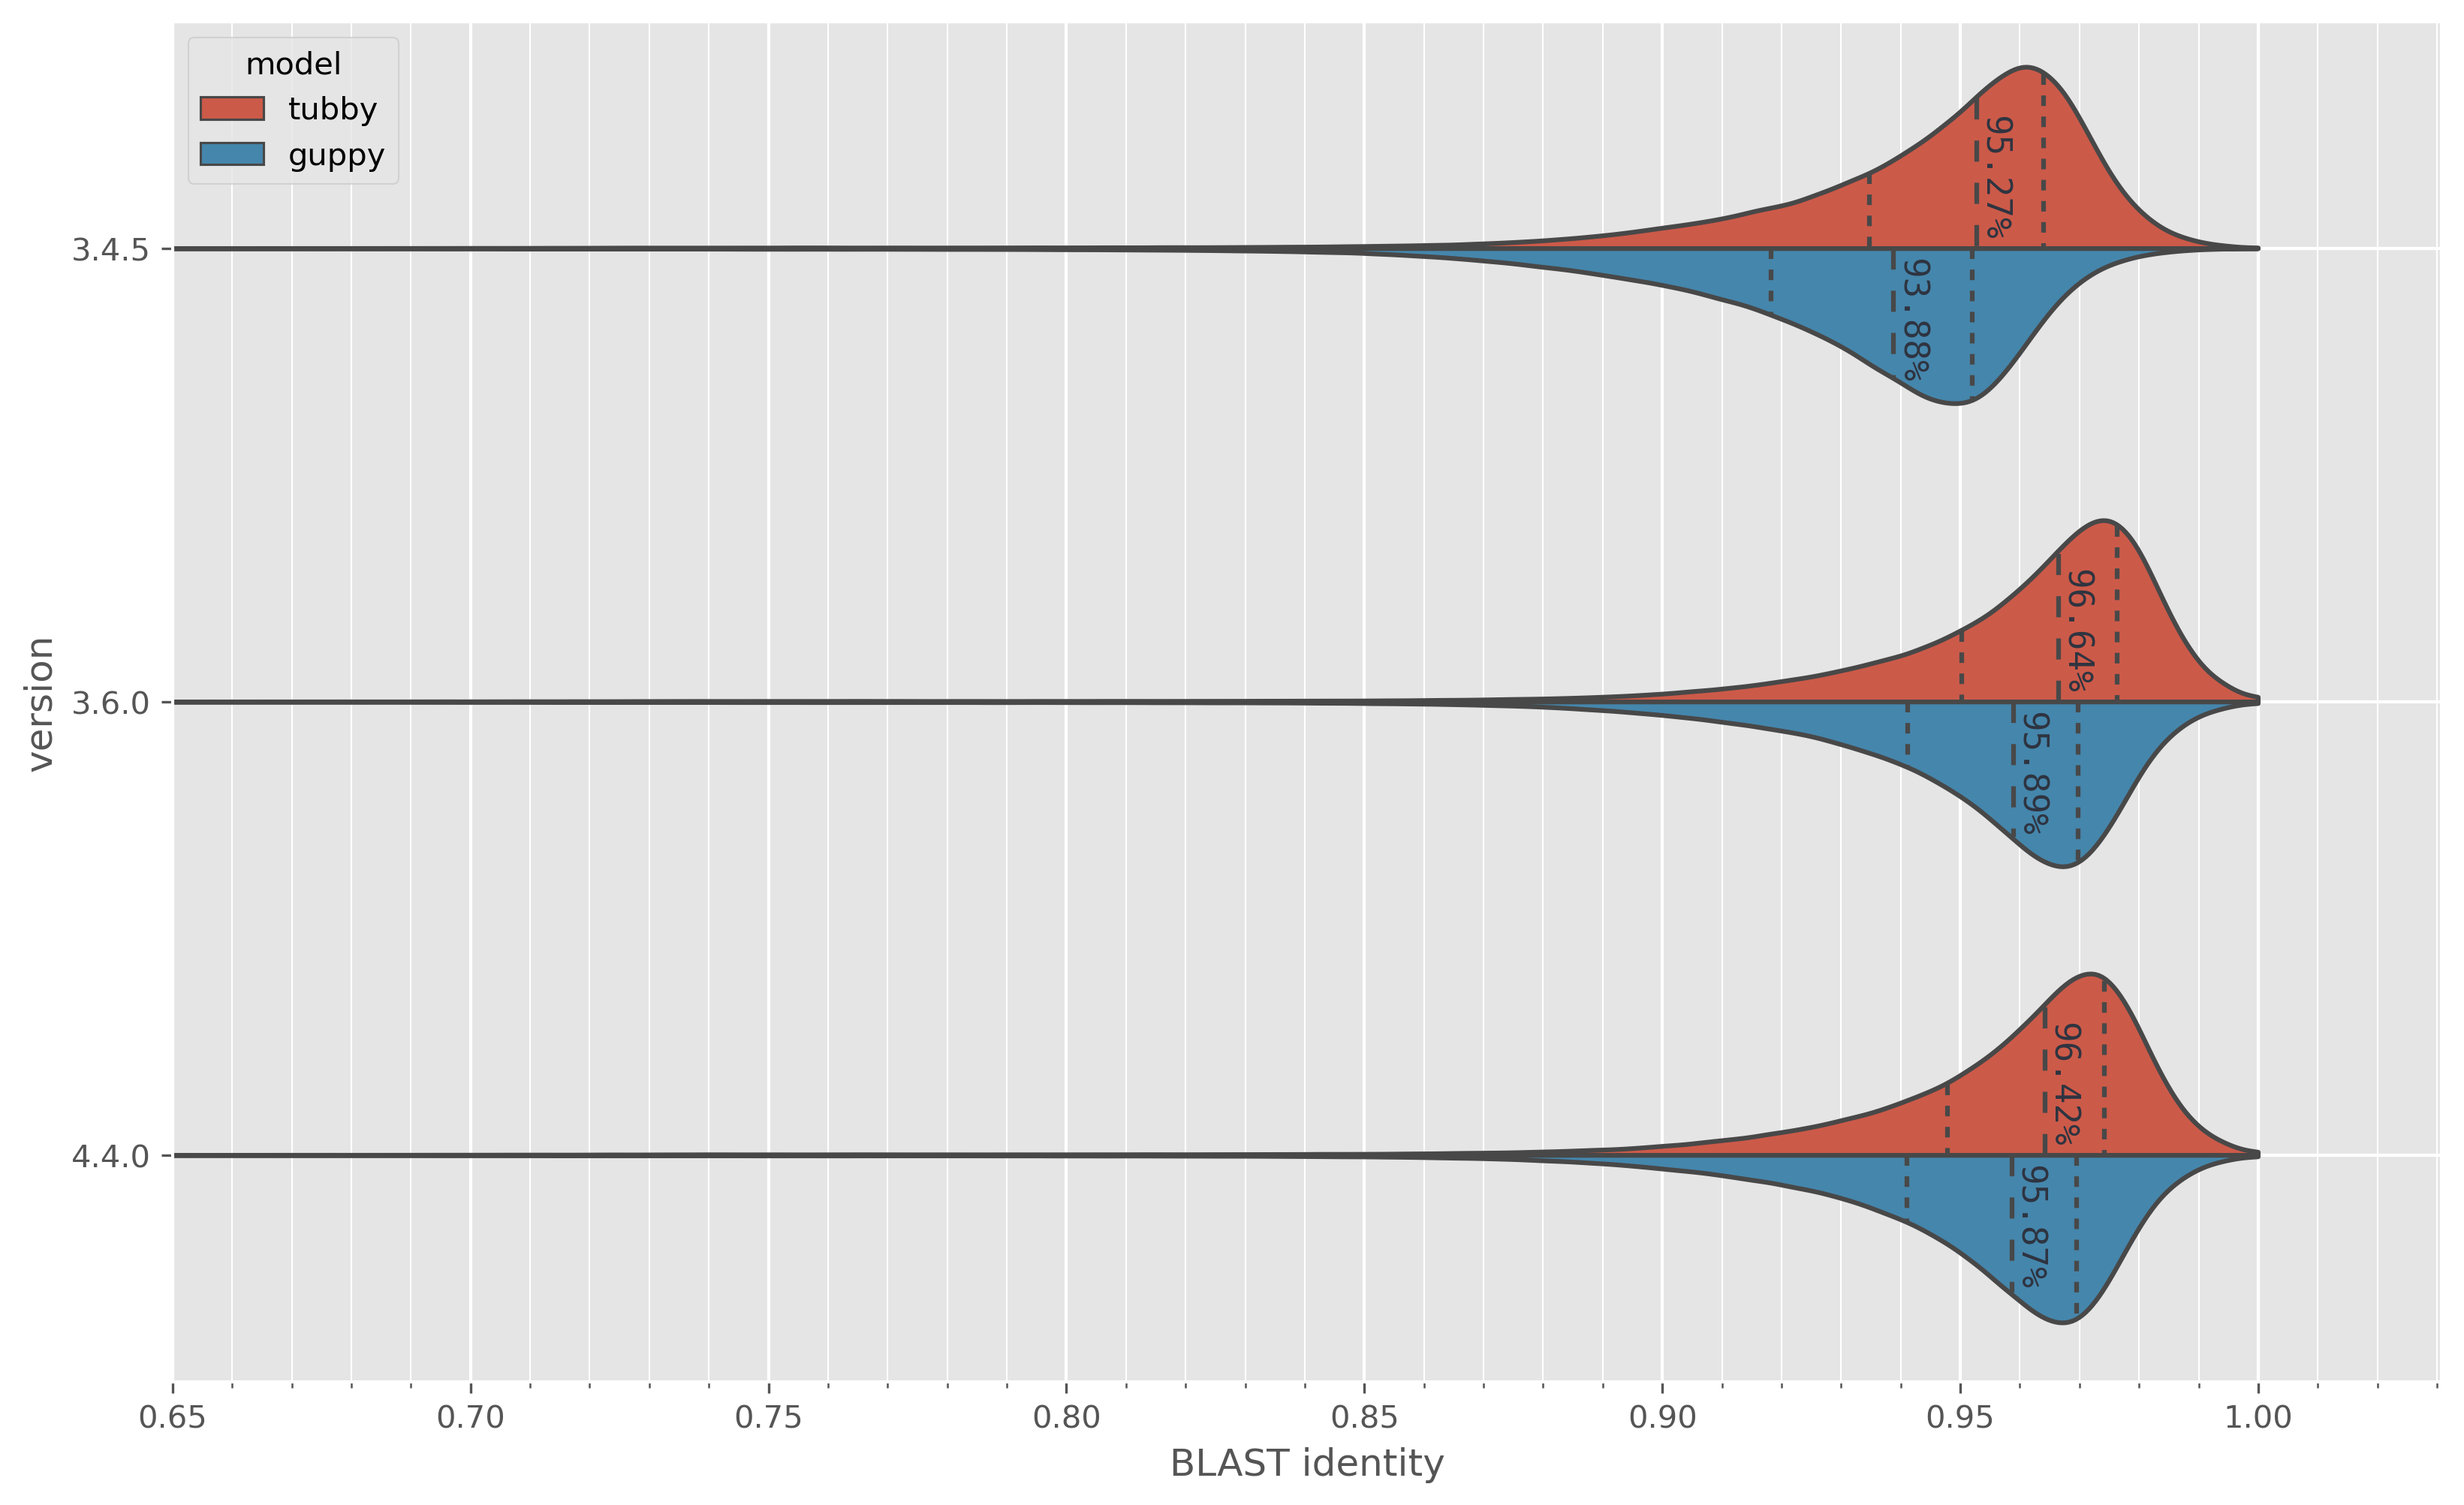
\includegraphics[width=1\linewidth]{Chapter4/Figs/test_read_blast_identity.png}
         \caption{Test data}
         \label{fig:test-read-blast}
     \end{subfigure}
    \caption{Read BLAST identity (x-axis) for the \mtb{}-specific basecalling model \tubby{} (red) compared with the default \guppy{} model (blue). The subtitle of each plot indicates the data being assessed. Version (y-axis) indicates the \guppy{} version used for the basecalling prior to, and after, training. BLAST identity is the number of matching bases (in a read alignment) divided by the length of the alignment. The median value for each violin is annotated on the middle dashed line.}
        \label{fig:read-blast}
\end{figure}

\begin{table}
\centering
\resizebox{\textwidth}{!}{%
\begin{tabular}{@{}llrrrrrrrrr@{}}
\toprule
Version                & Model & Count   & Mean   & std    & Min    & 25\%   & 50\%   & 75\%   & Max    & Mode    \\ \midrule
\multirow{2}{*}{3.4.5} & \guppy{} & 1047829 & 0.9067 & 0.0480 & 0.4186 & 0.8838 & 0.9202 & 0.9416 & 1.0000 & 0.9444 \\
                       & \tubby{} & 1047508 & 0.9295 & \textbf{0.0402} & 0.4619 & 0.9129 & 0.9415 & 0.9574 & 1.0000 & 0.9545 \\
\multirow{2}{*}{3.6.0} & \guppy{} & 1110664 & 0.9268 & 0.0474 & 0.4186 & 0.9063 & 0.9413 & 0.9604 & 1.0000 & 0.9615 \\
                       & \tubby{} & 1110098 & \textbf{0.9423} & 0.0413 & 0.4297 & \textbf{0.9269} & \textbf{0.9554} & \textbf{0.9704} & 1.0000 & \textbf{0.9688} \\
\multirow{2}{*}{4.4.0} & \guppy{} & 1144426 & 0.9247 & 0.0496 & \textbf{0.4751} & 0.9038 & 0.9403 & 0.9600 & 1.0000 & 0.9628 \\
                       & \tubby{} & 1143410 & 0.9381 & 0.0435 & 0.4723 & 0.9220 & 0.9520 & 0.9678 & 1.0000 & \textbf{0.9688} \\ \cmidrule(l){2-11} 
\end{tabular}%
}
\caption{Read BLAST identity summary statistics for the \mtb{}-specific basecalling model \tubby{} compared with the default \guppy{} model on the validation data. Version indicates the \guppy{} version used for the basecalling prior to, and after, training. BLAST identity is the number of matching bases (in a read alignment) divided by the length of the alignment. Count refers to the number of reads evaluated. std=standard deviation.}
\label{tab:read-blast}
\end{table}

\autoref{fig:eval-read-rel-len} shows that \tubby{} has a slight tendency towards deletions (shorter reads) compared to \guppy{}. However, this result is a little more complex than just looking at median values. The distribution of lengths for \guppy{} extends much further past 1.0 compared with \tubby{}, indicating an increase in insertions. We will return to this result when we look at the error types (\autoref{sec:tubby-error-types}). Summary statistics for the relative read lengths are shown in \autoref{tab:read-rel-len}.

\begin{figure}
     \centering
     \begin{subfigure}[b]{0.9\textwidth}
        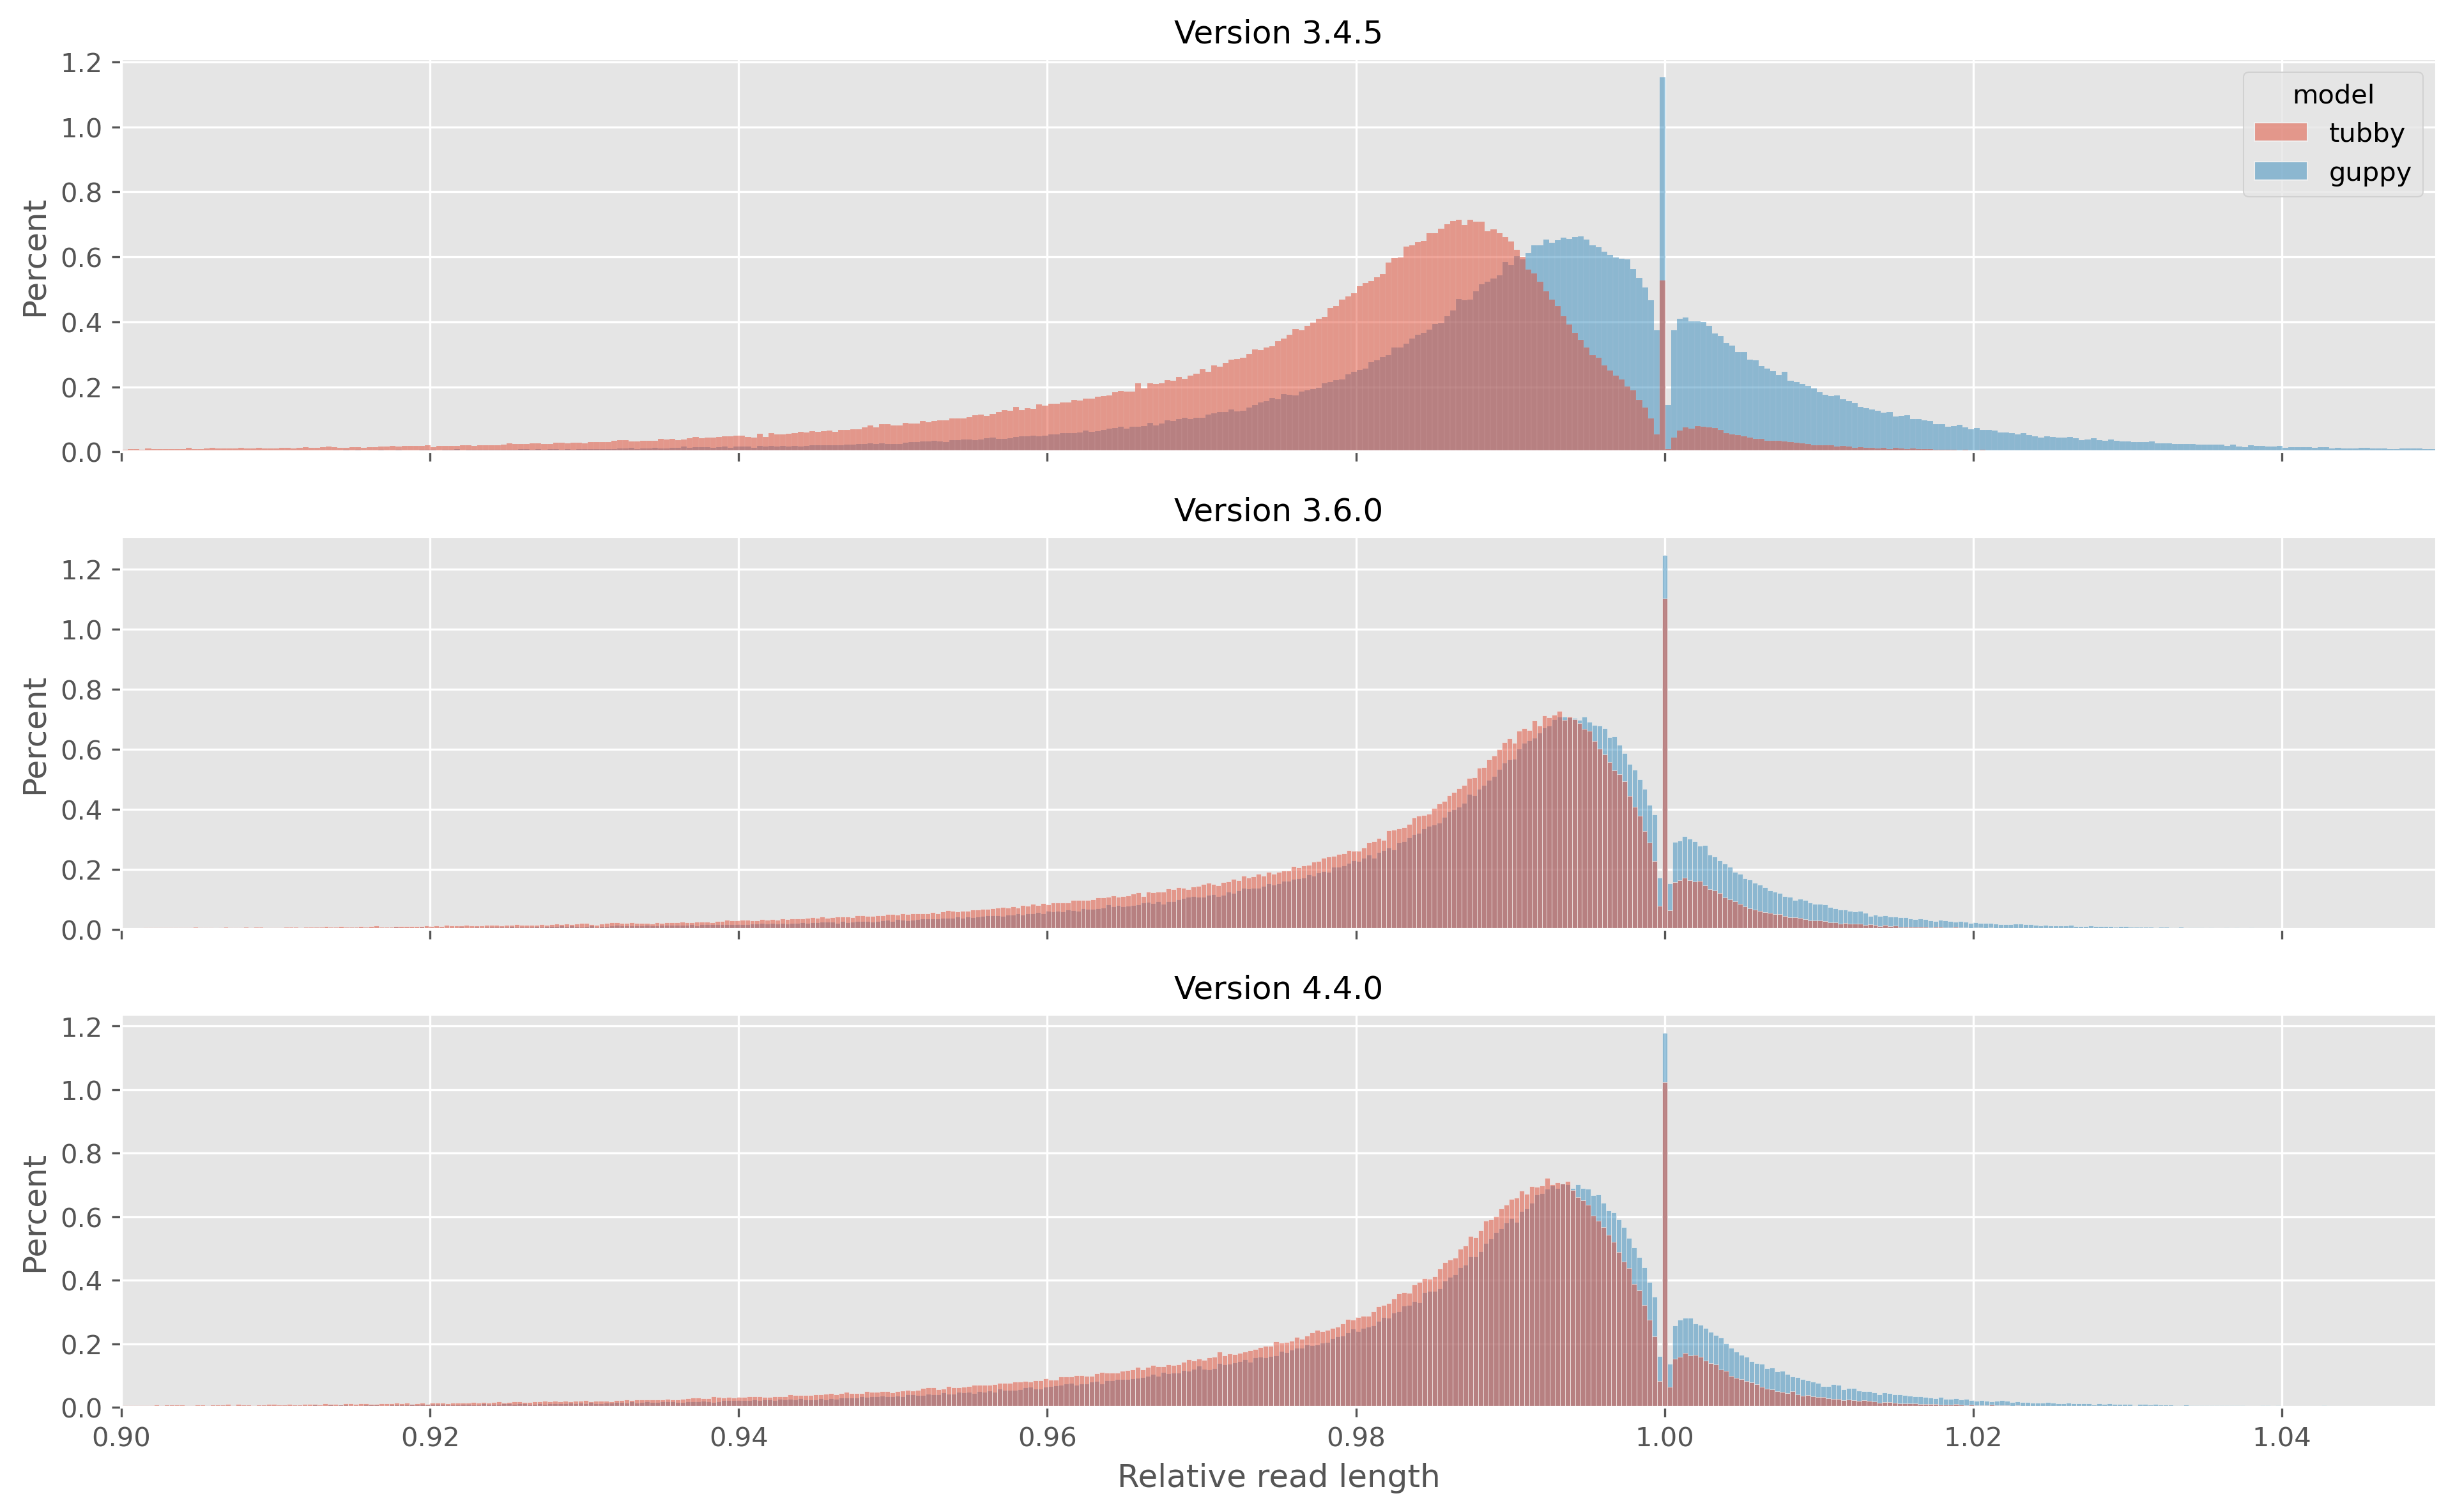
\includegraphics[width=1\linewidth]{Chapter4/Figs/read_rel_len.png}
        \centering
        \caption{Validation data}
        \label{fig:eval-read-rel-len}
     \end{subfigure}
     \hfill
     \begin{subfigure}[b]{0.9\textwidth}
         \centering
        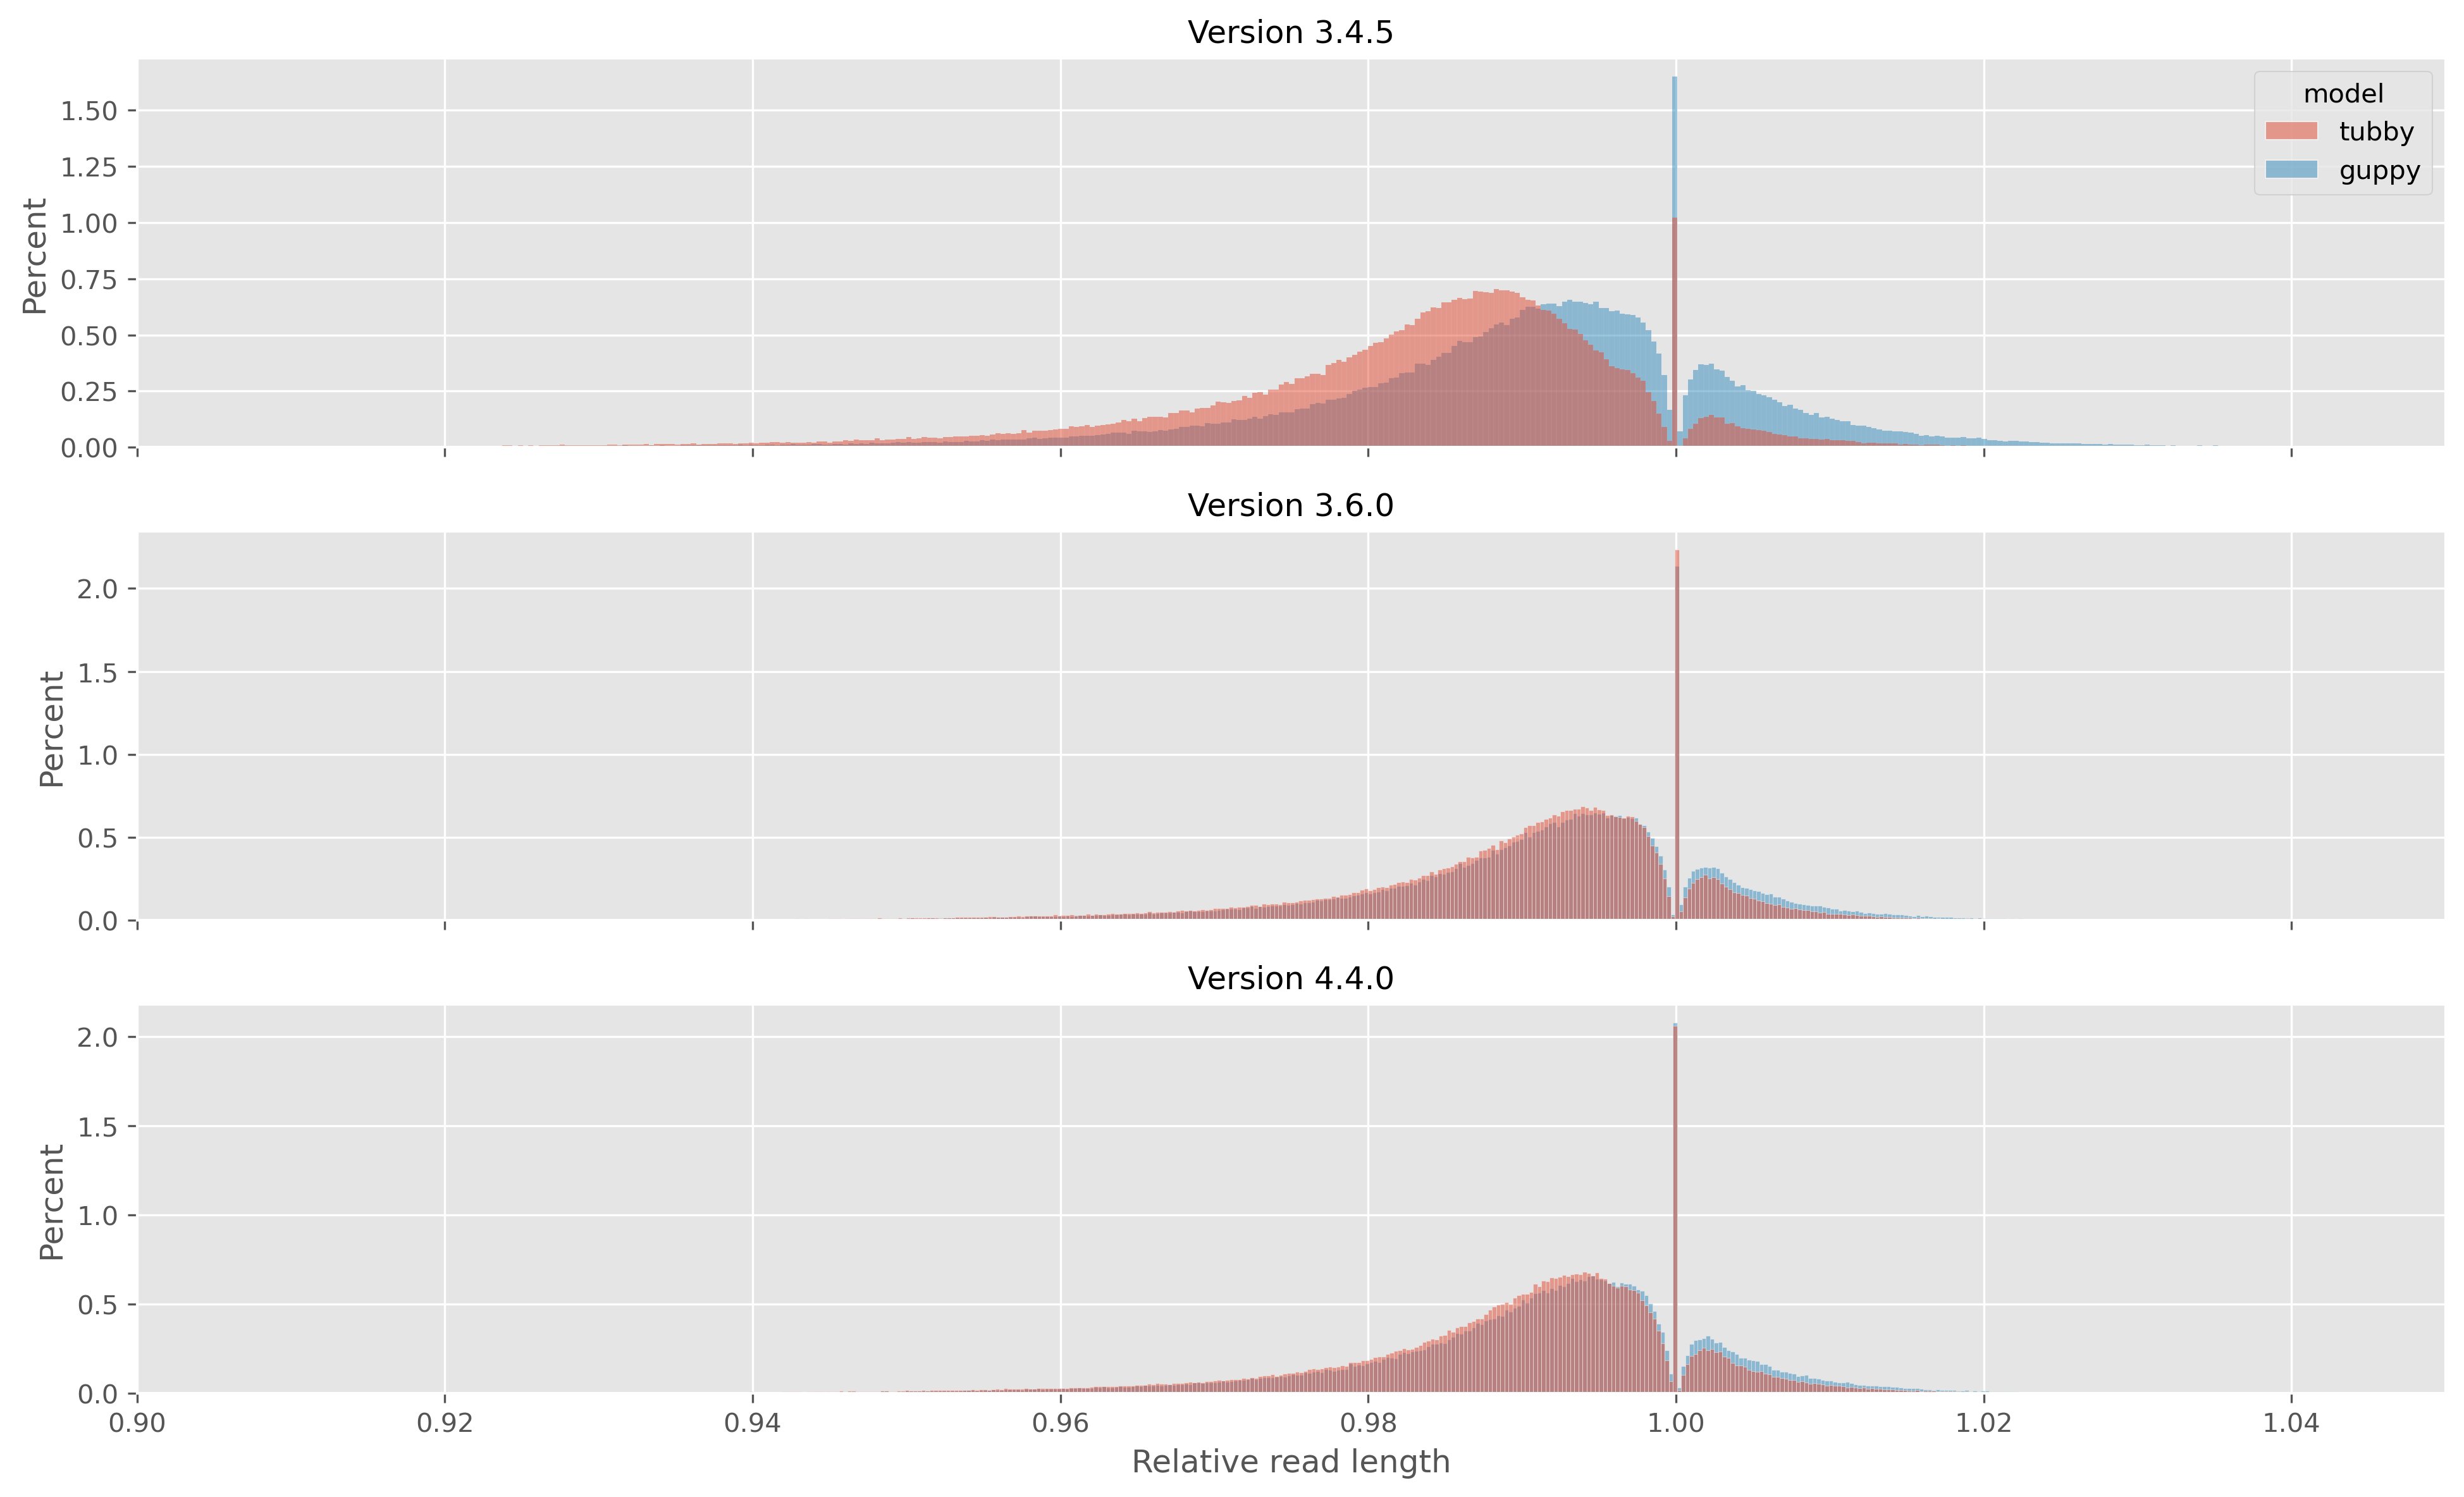
\includegraphics[width=1\linewidth]{Chapter4/Figs/test_read_rel_len.png}
         \caption{Test data}
         \label{fig:test-read-rel-len}
     \end{subfigure}
        \caption{Relative read length (y-axis) for the \mtb{}-specific basecalling model \tubby{} (red) compared with the default \guppy{} model (blue). The subtitle of each plot indicates the data being assessed. Relative read length is the length of the aligned part of the read, divided by the total length of the read. Version indicates the \guppy{} version used for the basecalling prior to, and after, training.}
        \label{fig:read-rel-len}
\end{figure}

\begin{table}
\centering
\resizebox{\textwidth}{!}{%
\begin{tabular}{@{}llrrrrrrrr@{}}
\toprule
Version                & Model & Count   & Mean   & std    & Min    & 25\%   & 50\%   & 75\%   & Max    \\ \midrule
\multirow{2}{*}{3.4.5} & \guppy{} & 1047829 & 0.9919 & 0.0240 & 0.4558 & 0.9842 & 0.9932 & 1.0014 & 1.9881 \\
                       & \tubby{} & 1047508 & 0.9764 & 0.0239 & 0.4936 & 0.9698 & 0.9822 & 0.9892 & 1.8949 \\
\multirow{2}{*}{3.6.0} & \guppy{} & 1110664 & 0.9873 & 0.0233 & 0.4495 & 0.9819 & 0.9914 & 0.9974 & 2.0322 \\
                       & \tubby{} & 1110098 & 0.9817 & 0.0241 & 0.4531 & 0.9761 & 0.9882 & 0.9943 & 1.9031 \\
\multirow{2}{*}{4.4.0} & \guppy{} & 1144426 & 0.9862 & 0.0241 & 0.5085 & 0.9806 & 0.9907 & 0.9969 & 1.9146 \\
                       & \tubby{} & 1143410 & 0.9814 & 0.0246 & 0.4963 & 0.9758 & 0.9879 & 0.9941 & 1.8851 \\ \cmidrule(l){2-10} 
\end{tabular}%
}
\caption{Relative read length for the \mtb{}-specific basecalling model \tubby{} compared with the default \guppy{} model on the validation data. Relative read length is the length of the aligned part of the read, divided by the total length of the read. Version indicates the \guppy{} version used for the basecalling prior to, and after, training. Count refers to the number of reads evaluated. std=standard deviation.}
\label{tab:read-rel-len}
\end{table}

\subsubsection{Test data}

\autoref{fig:test-read-blast} shows the read BLAST identities for the test BCG sample. As with the validation data, version 3.6.0 \tubby{} has the highest median read identity of 96.64\% - 1.10\% greater than the validation data. From \autoref{tab:test-read-blast}, we see that \tubby{} version 3.6.0 has the highest percentiles, mode (97.67\%), and mean (95.87\%) of all the models and versions.

Again, for each version, \tubby{} outperforms \guppy{} on all summary statistics (except the mode for version 4.4.0, which is the same).

\begin{table}
\centering
\resizebox{\textwidth}{!}{%
\begin{tabular}{@{}llrrrrrrrrr@{}}
\toprule
Version                & Model & Count   & Mean   & std    & Min    & 25\%   & 50\%   & 75\%   & Max    & Mode    \\ \midrule
\multirow{2}{*}{3.4.5} & \guppy{} & 787170 & 0.9309 & 0.0330          & 0.4738 & 0.9183 & 0.9388 & 0.9520 & 1.0000 & 0.9444 \\
                       & \tubby{} & 790230 & 0.9453 & 0.0308          & 0.4764 & 0.9348 & 0.9527 & 0.9640 & 1.0000 & 0.9545 \\
\multirow{2}{*}{3.6.0} & \guppy{} & 791527 & 0.9509 & 0.0321          & 0.3841 & 0.9412 & 0.9589 & 0.9698 & 1.0000 & 0.9688 \\
 & \tubby{} & 791356 & \textbf{0.9587} & 0.0307 & \textbf{0.4819} & \textbf{0.9502} & \textbf{0.9664} & \textbf{0.9763} & 1.0000 & \textbf{0.9767} \\
\multirow{2}{*}{4.4.0} & \guppy{} & 790291 & 0.9507 & 0.0318          & 0.4328 & 0.9411 & 0.9587 & 0.9695 & 1.0000 & 0.9688 \\
                       & \tubby{} & 791217 & 0.9566 & \textbf{0.0305} & 0.3915 & 0.9479 & 0.9642 & 0.9742 & 1.0000 & 0.9688 \\ \cmidrule(l){2-11} 
\end{tabular}%
}
\caption{Read BLAST identity summary statistics for the \mtb{}-specific basecalling model \tubby{} compared with the default \guppy{} model on the test data. Version indicates the \guppy{} version used for the basecalling prior to, and after, training. BLAST identity is the number of matching bases (in a read alignment) divided by the length of the alignment. Count refers to the number of reads evaluated. std=standard deviation.}
\label{tab:test-read-blast}
\end{table}

The relative read length distributions show in \autoref{fig:test-read-rel-len} indicate that on the test data, \tubby{} and \guppy{} have the same slight tendency towards deletions (shorter reads). However, both models have much similar relative read lengths to each other when compared to the validation data - except version 3.4.5. Summary statistics for the relative read lengths are shown in \autoref{tab:test-read-rel-len}.

\begin{table}
\centering
\resizebox{\textwidth}{!}{%
\begin{tabular}{@{}llllllllll@{}}
\toprule
Version                & Model & Count   & Mean   & std    & Min    & 25\%   & 50\%   & 75\%   & Max    \\ \midrule
\multirow{2}{*}{3.4.5} & \guppy{} & 787170 & 0.990146 & 0.020453 & 0.507716 & 0.983563 & 0.991832 & 0.998854 & 1.885660 \\
                       & \tubby{} & 790230 & 0.982657 & 0.020303 & 0.512180 & 0.976847 & 0.985492 & 0.991870 & 2.011945 \\
\multirow{2}{*}{3.6.0} & \guppy{} & 791527 & 0.990858 & 0.019202 & 0.516049 & 0.986090 & 0.993108 & 0.998485 & 2.519333 \\
                       & \tubby{} & 791356 & 0.989297 & 0.019148 & 0.519136 & 0.984899 & 0.992054 & 0.997132 & 2.017065 \\
\multirow{2}{*}{4.4.0} & \guppy{} & 790291 & 0.990601 & 0.019214 & 0.515123 & 0.985816 & 0.992832 & 0.998220 & 2.137884 \\
                       & \tubby{} & 791217 & 0.989091 & 0.019307 & 0.514339 & 0.984615 & 0.991718 & 0.996894 & 2.525117 \\ \cmidrule(l){2-10} 
\end{tabular}%
}
\caption{Relative read length for the \mtb{}-specific basecalling model \tubby{} compared with the default \guppy{} model on the test data. Relative read length is the length of the aligned part of the read, divided by the total length of the read. Version indicates the \guppy{} version used for the basecalling prior to, and after, training. Count refers to the number of reads evaluated. std=standard deviation.}
\label{tab:test-read-rel-len}
\end{table}

% =====
\subsection{Consensus-level performance}

To assess consensus-level accuracy of each model, we require assemblies from the basecalled reads. However, to allow for comparison of these model-specific consensus sequences (assemblies) to the truth assembly, a reference-guided method is needed to ensure overall structure of the truth and consensus sequences is the same. We use Rebaler (version 0.2.0; \url{https://github.com/rrwick/Rebaler}), a tool developed for exactly this use-case \cite{wick2019}. Briefly, \vrb{rebaler} aligns the reads to a reference sequence and replaces that sequence with the sequence from the best alignments, producing an unpolished assembly. After this, it polishes the assembly with \vrb{racon} to produce a consensus sequence. 

We then use the same approach as in \cite{wick2020} to quantify the similarity of the consensus and truth assemblies for each sample. Each contig (chromosome) in the consensus assembly in aligned to the truth assembly with \vrb{minimap2}. We calculate the chromosome identity for each contig's longest alignment in the same fashion as BLAST identity (\autoref{sec:tubby-read}).

\subsubsection{Validation data}

\autoref{fig:eval-chrom-identity} shows the chromosome identity for each version and model. We again see that \tubby{} version 3.6.0 leads to the highest identity values, with a median chromosome identity value of 99.96\%. Compared to the best median \guppy{} identity of 99.94\% (version 3.6.0), \tubby{} provides an improvement of 0.02\%, which equates to approximately 880 less erroneous positions in the \mtb{} assembly.

\begin{figure}
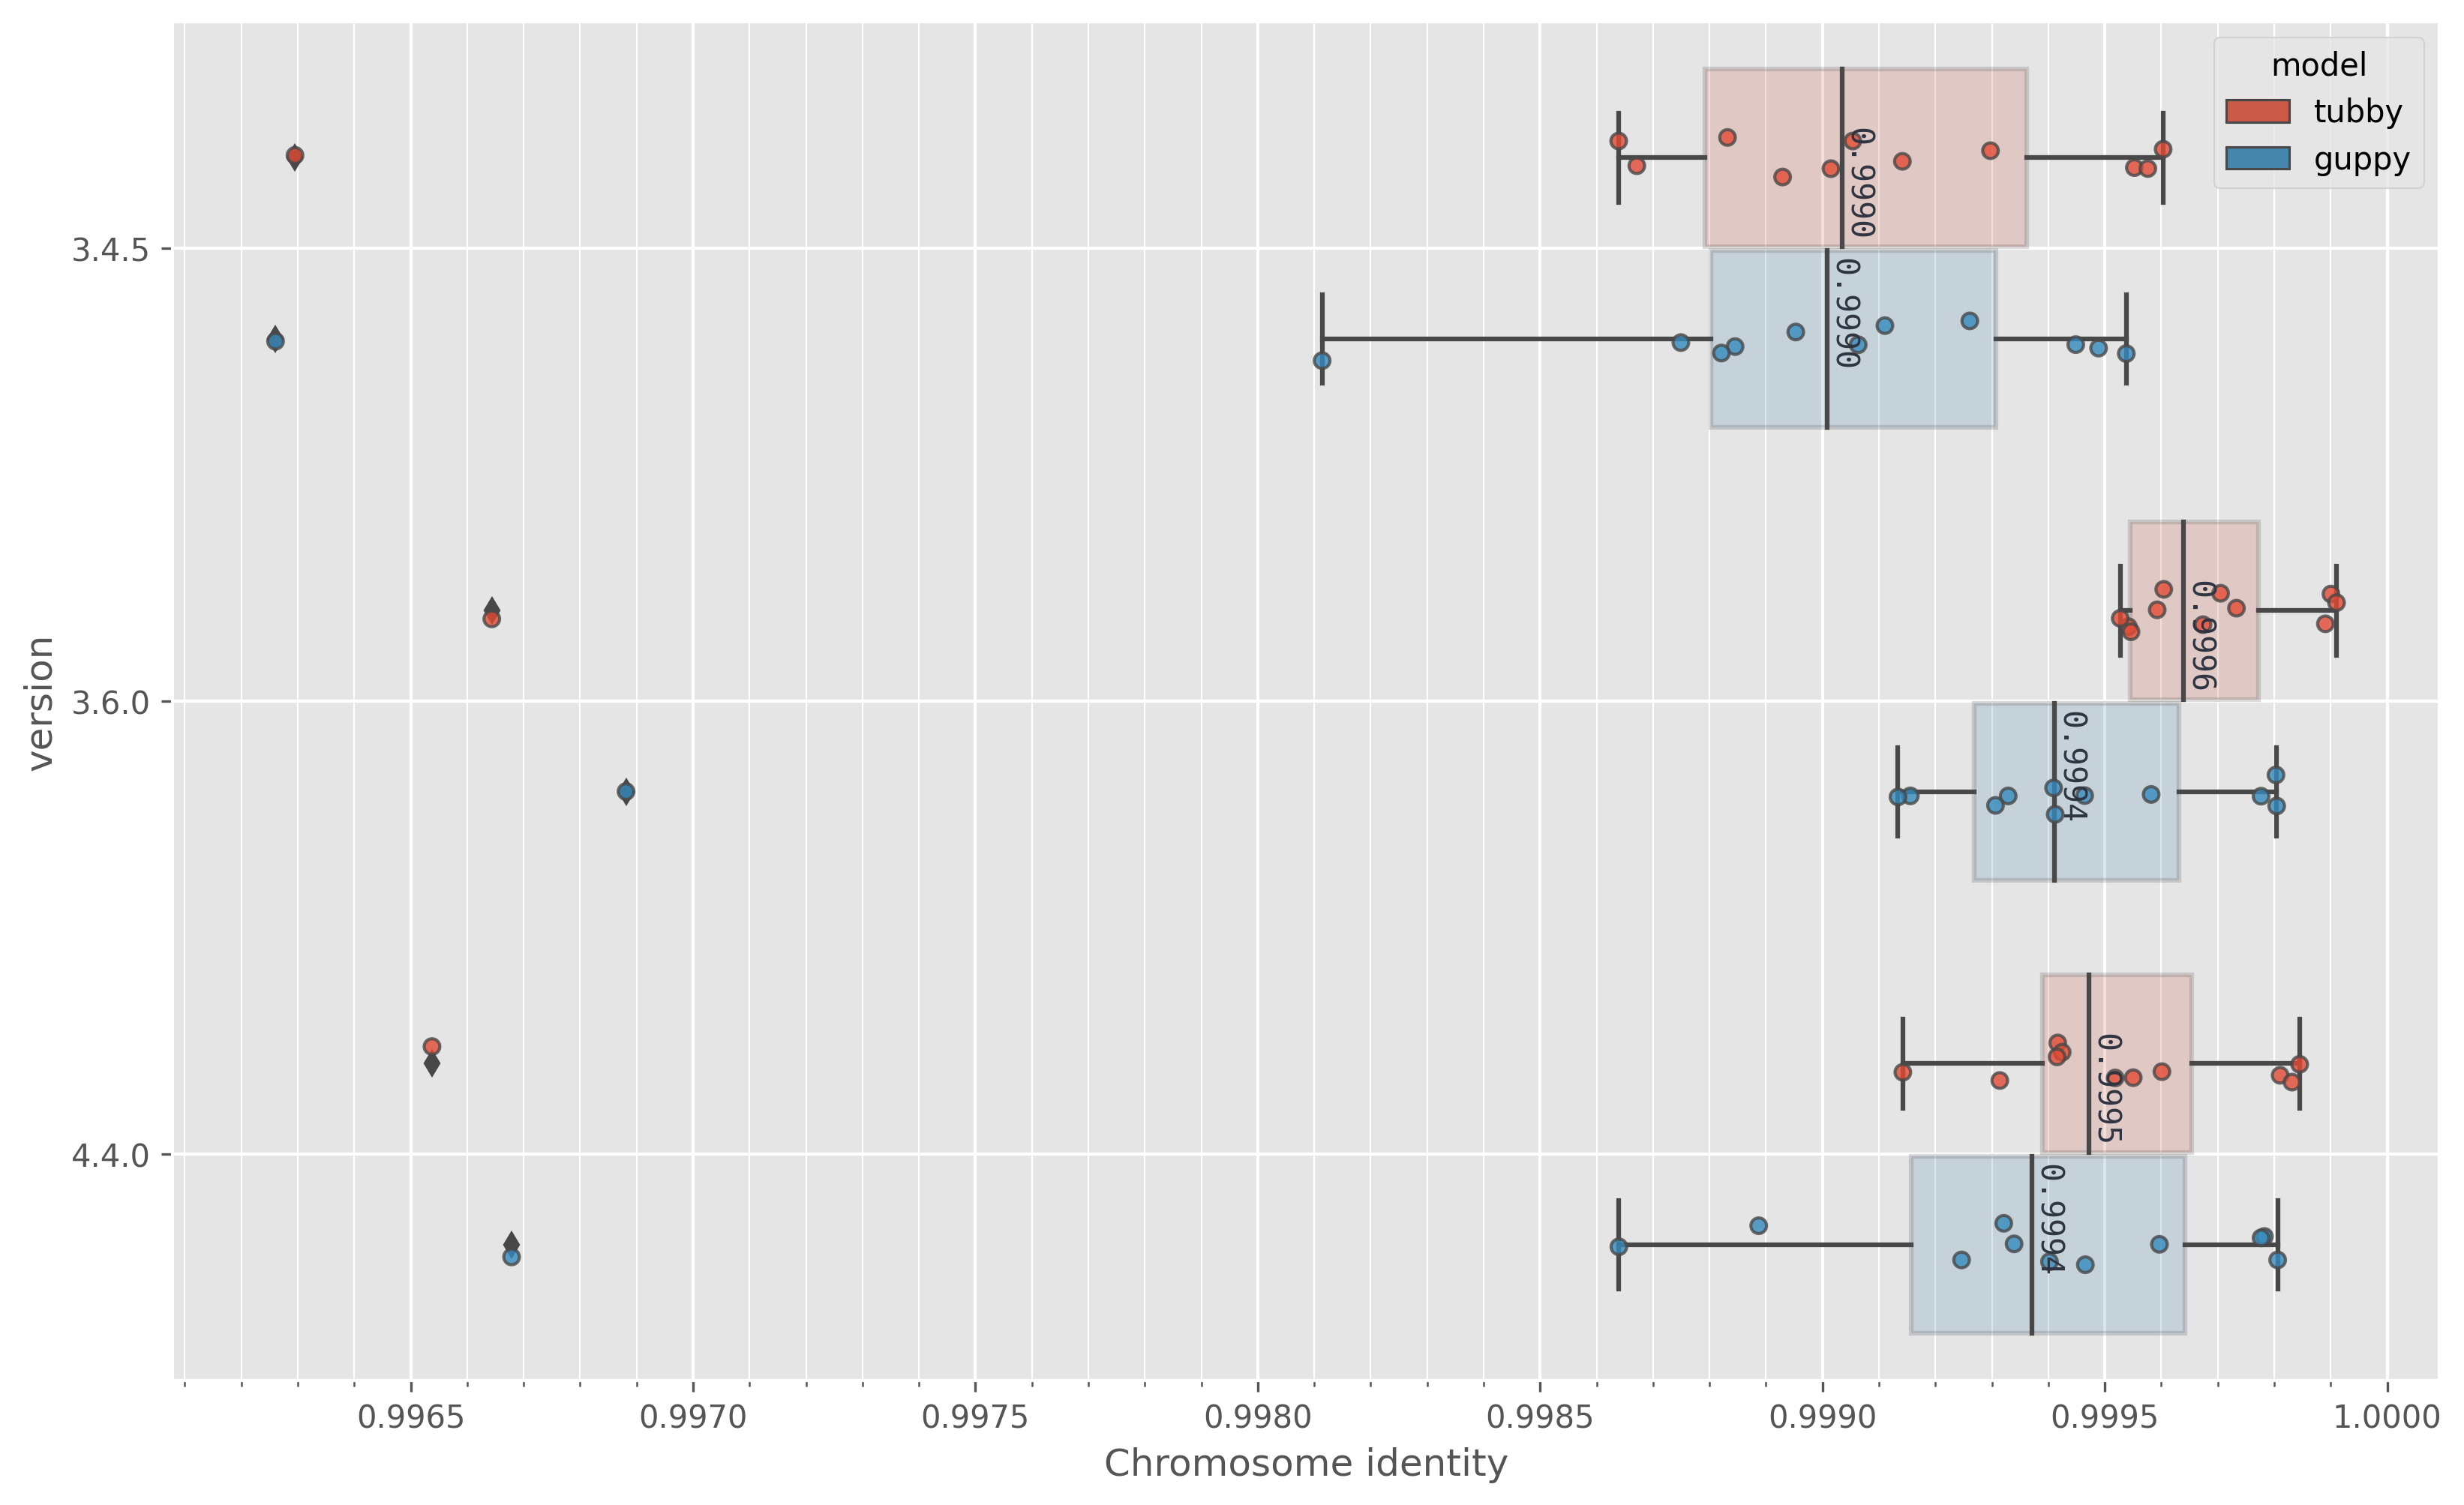
\includegraphics[width=0.9\textwidth]{Chapter4/Figs/eval_chromosome_identity.png}
\centering
\caption{Chromosome identity (x-axis) for the \mtb{}-specific basecalling model \tubby{} (red) compared with the default \guppy{} model (blue) on the validation data. Version (y-axis) indicates the \guppy{} version used for the basecalling prior to, and after, training. For each chromosome's longest alignment to its truth assembly, chromosome identity is the number of matching bases divided by the length of the alignment. The coloured points indicate the individual chromosome identity for each contig in each sample.}
\label{fig:eval-chrom-identity}
\end{figure}

\begin{table}
\centering
\resizebox{\textwidth}{!}{%
\begin{tabular}{@{}llrrrrrrrr@{}}
\toprule
Version                & Model & Contigs & Mean   & std    & Min    & 25\%   & 50\%   & 75\%   & Max    \\ \midrule
\multirow{2}{*}{3.4.5} & \guppy{} & 12      & 0.9988 & 0.0009 & 0.9963 & 0.9988 & 0.9990 & 0.9993 & 0.9995 \\
                       & \tubby{} & 12      & 0.9989 & 0.0009 & 0.9963 & 0.9988 & 0.9990 & 0.9994 & 0.9996 \\
\multirow{2}{*}{3.6.0} & \guppy{} & 12      & 0.9993 & \textbf{0.0008} & \textbf{0.9969} & 0.9993 & 0.9994 & 0.9996 & 0.9998 \\
                       & \tubby{} & 12      & \textbf{0.9994} & 0.0009 & 0.9966 & \textbf{0.9995} & \textbf{0.9996} & \textbf{0.9998} & \textbf{0.9999} \\
\multirow{2}{*}{4.4.0} & \guppy{} & 12      & 0.9992 & 0.0009 & 0.9967 & 0.9992 & 0.9994 & 0.9996 & 0.9998 \\
                       & \tubby{} & 12      & 0.9993 & 0.0009 & 0.9965 & 0.9994 & 0.9995 & 0.9997 & 0.9998 \\ \cmidrule(l){2-10} 
\end{tabular}%
}
\caption{Chromosome identity for the \mtb{}-specific basecalling model \tubby{} compared with the default \guppy{} model on the validation data. Version indicates the \guppy{} version used for the basecalling prior to, and after, training. For each chromosome's longest alignment to its truth assembly, chromosome identity is the number of matching bases divided by the length of the alignment. std=standard deviation.}
\label{tab:eval-chrom-identity}
\end{table}

% In addition to the chromosome identity, we also investigate the longest indel in each consensus assembly. Large-scale indels are much harder to fix via polishing
% The maximum indel length is taken from each chromosome's longest alignment to its truth assembly. maximum indel length is the CIGAR string insertion (I) or deletion (D) operation with the largest value.

% \begin{figure}
% 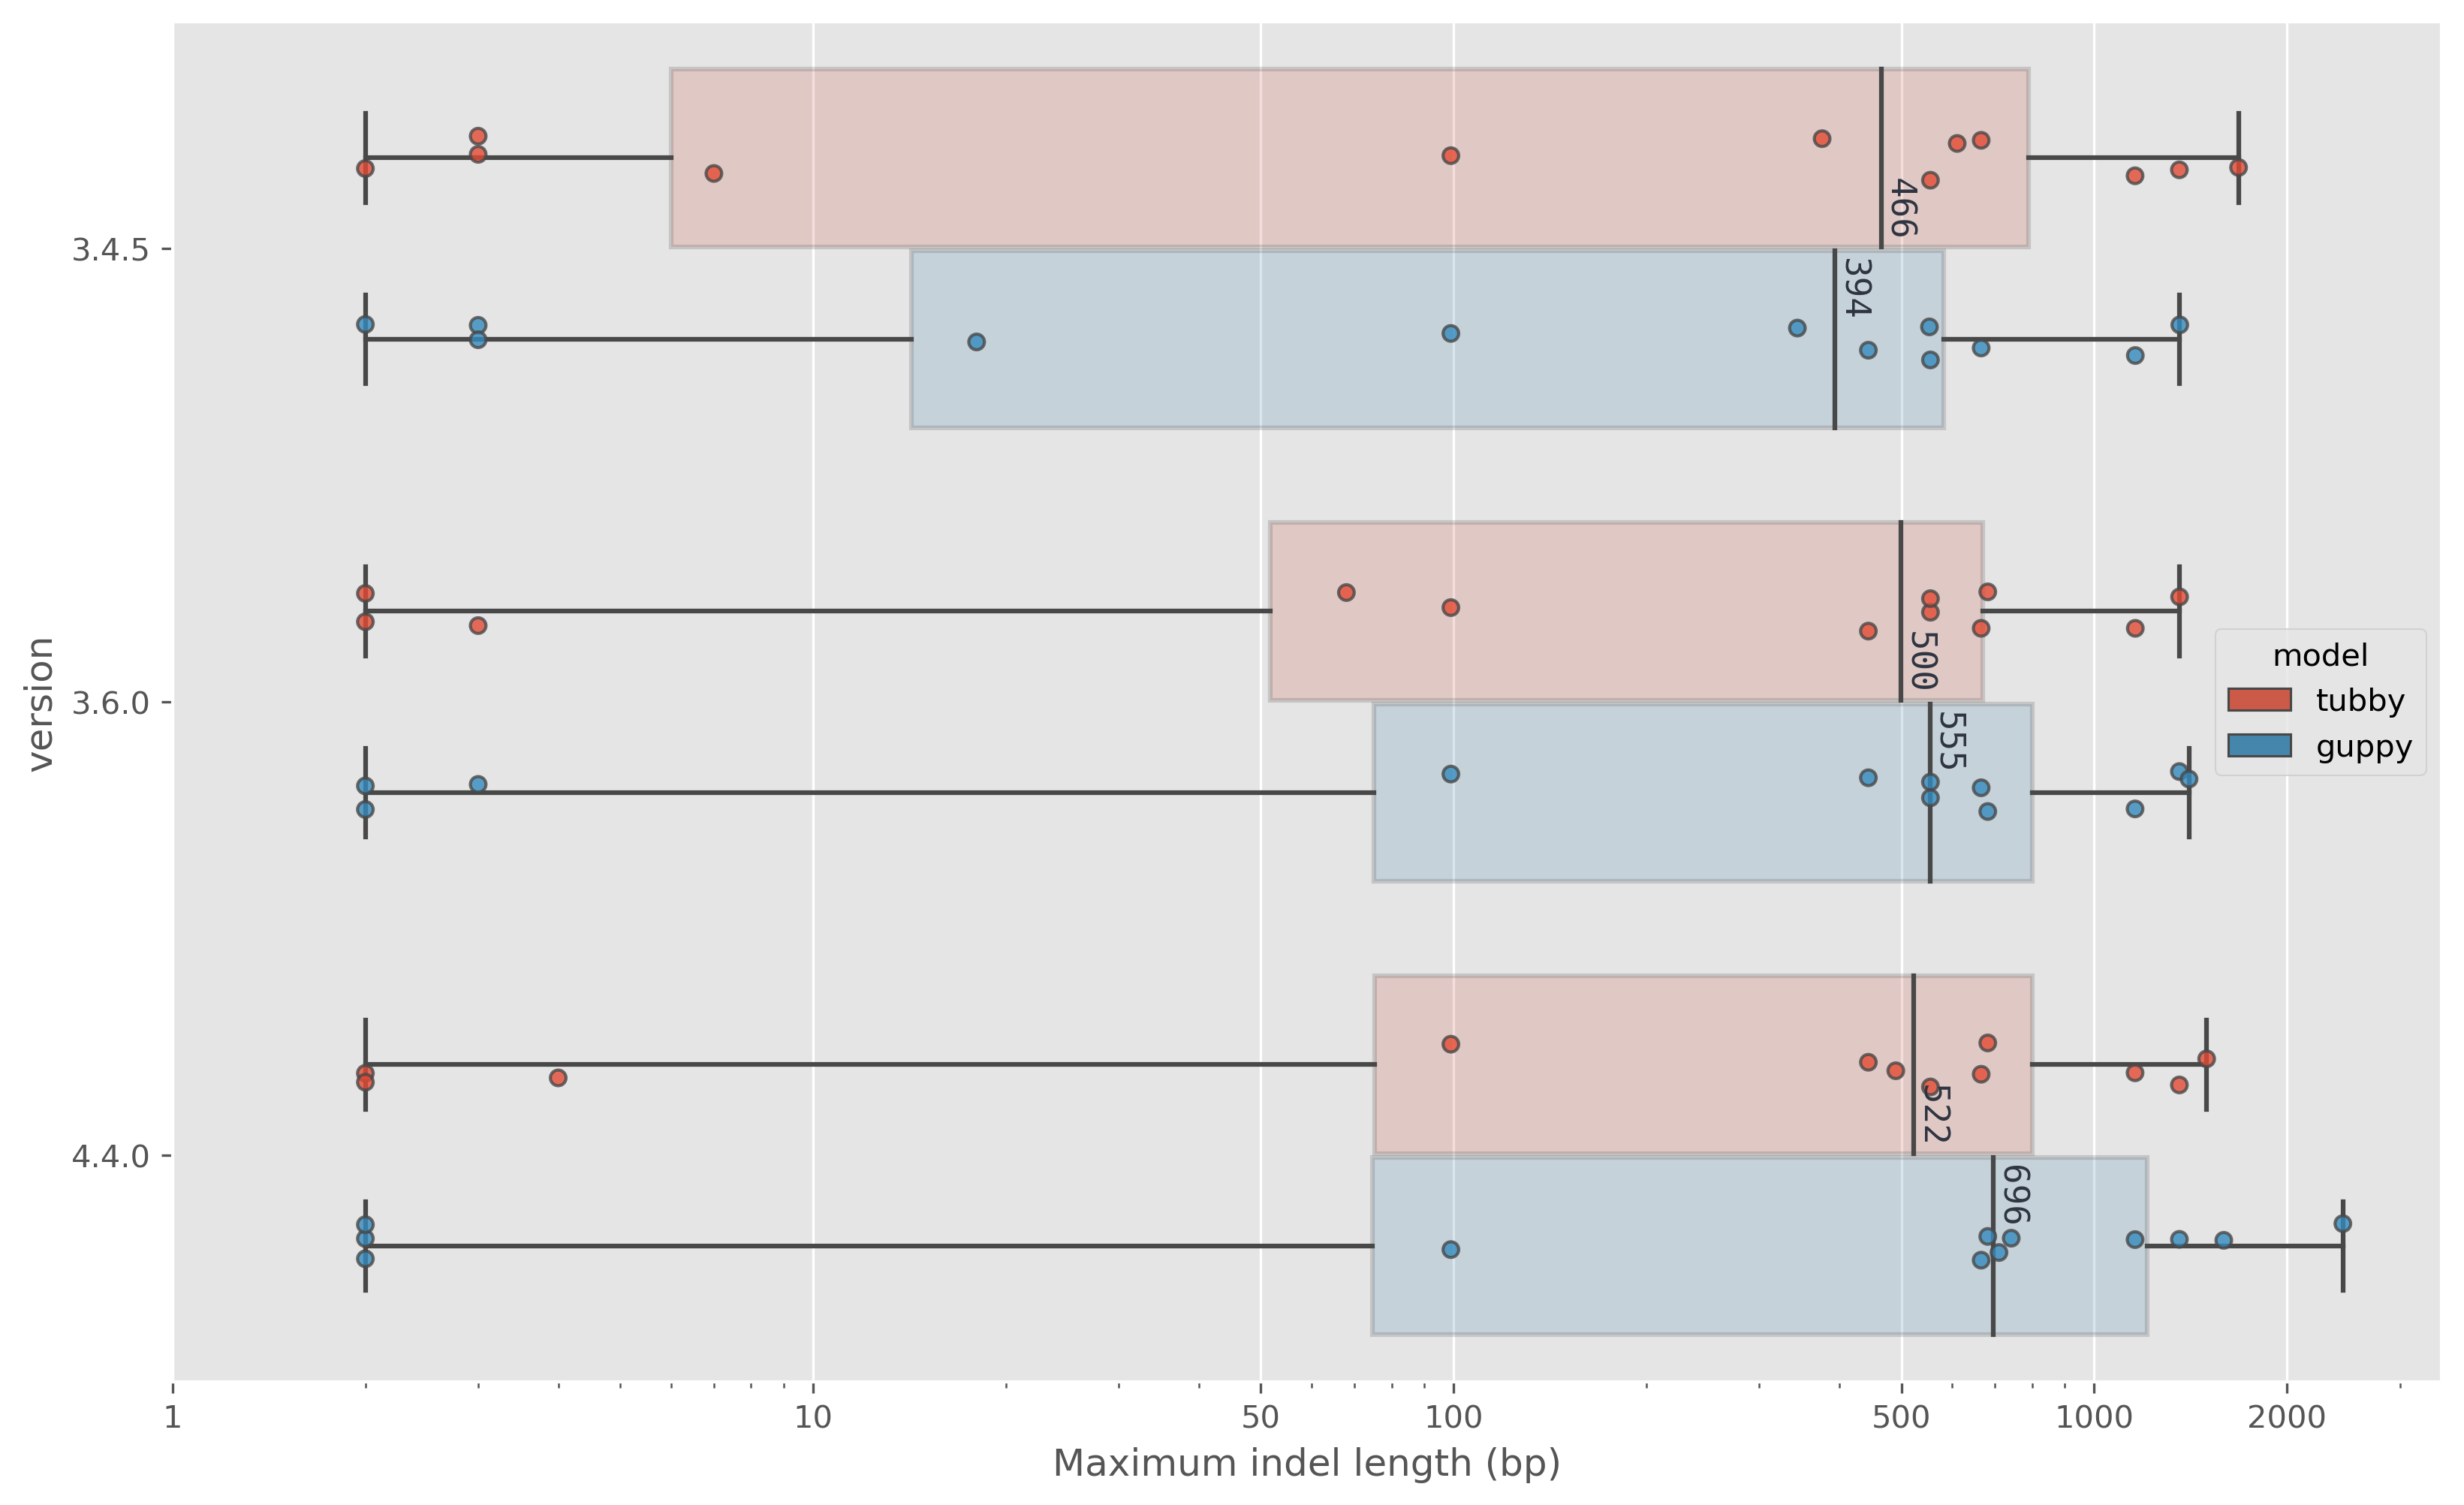
\includegraphics[width=0.9\textwidth]{Chapter4/Figs/eval_max_indel.png}
% \centering
% \caption{Maximum indel length (x-axis) for the \mtb{}-specific basecalling model \tubby{} (red) compared with the default \guppy{} model (blue). Version (y-axis) indicates the \guppy{} version used for the basecalling prior to, and after, training. The maximum indel length is taken from each chromosome's longest alignment to its truth assembly. The coloured points indicate the individual values for each contig in each sample.}
% \label{fig:eval-max-indel}
% \end{figure}

\subsubsection{Test data}

Each basecalling model and version produced a single contig for the BCG test sample. These values are listed in \autoref{tab:test-chrom-identity}, where we see \tubby{} version 3.6.0 produces the highest chromosome identity of 99.11\%. This is a lot lower than the median value of 99.96\% obtained on the validation data; it is even less than the minimum chromosome identity for any validation data consensus assembly (99.63\%; \autoref{tab:eval-chrom-identity}).

\begin{table}
\centering
\begin{tabular}{@{}lllllll@{}}
\toprule
Version  & \multicolumn{2}{l}{3.4.5} & \multicolumn{2}{l}{3.6.0} & \multicolumn{2}{l}{4.4.0} \\ \midrule
Model    & \guppy{}       & \tubby{}       & \guppy{}        & \tubby{}       & \guppy{}        & \tubby{}       \\
Identity & 0.9886      & 0.9878      & 0.9881      & \textbf{0.9911}      & 0.9883      & 0.9884      \\ \bottomrule
\end{tabular}
\caption{Chromosome identity for the \mtb{}-specific basecalling model \tubby{} compared with the default \guppy{} model on the BCG test sample. Version indicates the \guppy{} version used for the basecalling prior to, and after, training. For each chromosome's longest alignment to its truth assembly, chromosome identity is the number of matching bases divided by the length of the alignment.}
\label{tab:test-chrom-identity}
\end{table}

% ====
\subsection{Error types}
\label{sec:tubby-error-types}

Lastly, we classify the the types of errors that occur in the assemblies produced from each model's output. The \vrb{rebaler} assembly for each model and sample combination was aligned to the sample's truth assembly using `nucmer`(CITE). `nucmer` produces all positions of difference - errors in this case - between the two sequences. We classify errors as Dcm if the reported difference occurs in a known 5-methylcystosine methyltransferases motif(CITE), homopolymer insertion or deletion if the difference involves as base being added/removed from a region containing 3 or more of that same base. All deletions, insertions, and substitutions that do not fit into one of these categories after reported in their own group.

Here we classify the types of errors that occur in the \vrb{rebaler} assemblies and look at how these errors compare across models. To determine the errors, we categorise the differences between the truth and \vrb{rebaler} assemblies (see \todo{link to relevant methods}). \autoref{fig:error_types} shows that the greater part of the error types (for both models) are attributable to deletions, with most being homopolymer deletions. We do however see that, except for non-homopolymer deletions, tubby's errors are lower than \guppy{}'s \todo{add some concrete numbers}. In the case of both insertion types, tubby has approximately 3.5-fold less insertions than \guppy{} - although these constitute a small portion of the overall errors. Both models have a very low level of Dcm-methylation errors, which is a nice control of sorts as \mtb{} does not have any known 5-methylcystosine methyltransferases(CITE)\improvement{ensure the wording of this and correct and that the claim is also correct}.

% \begin{figure}
% 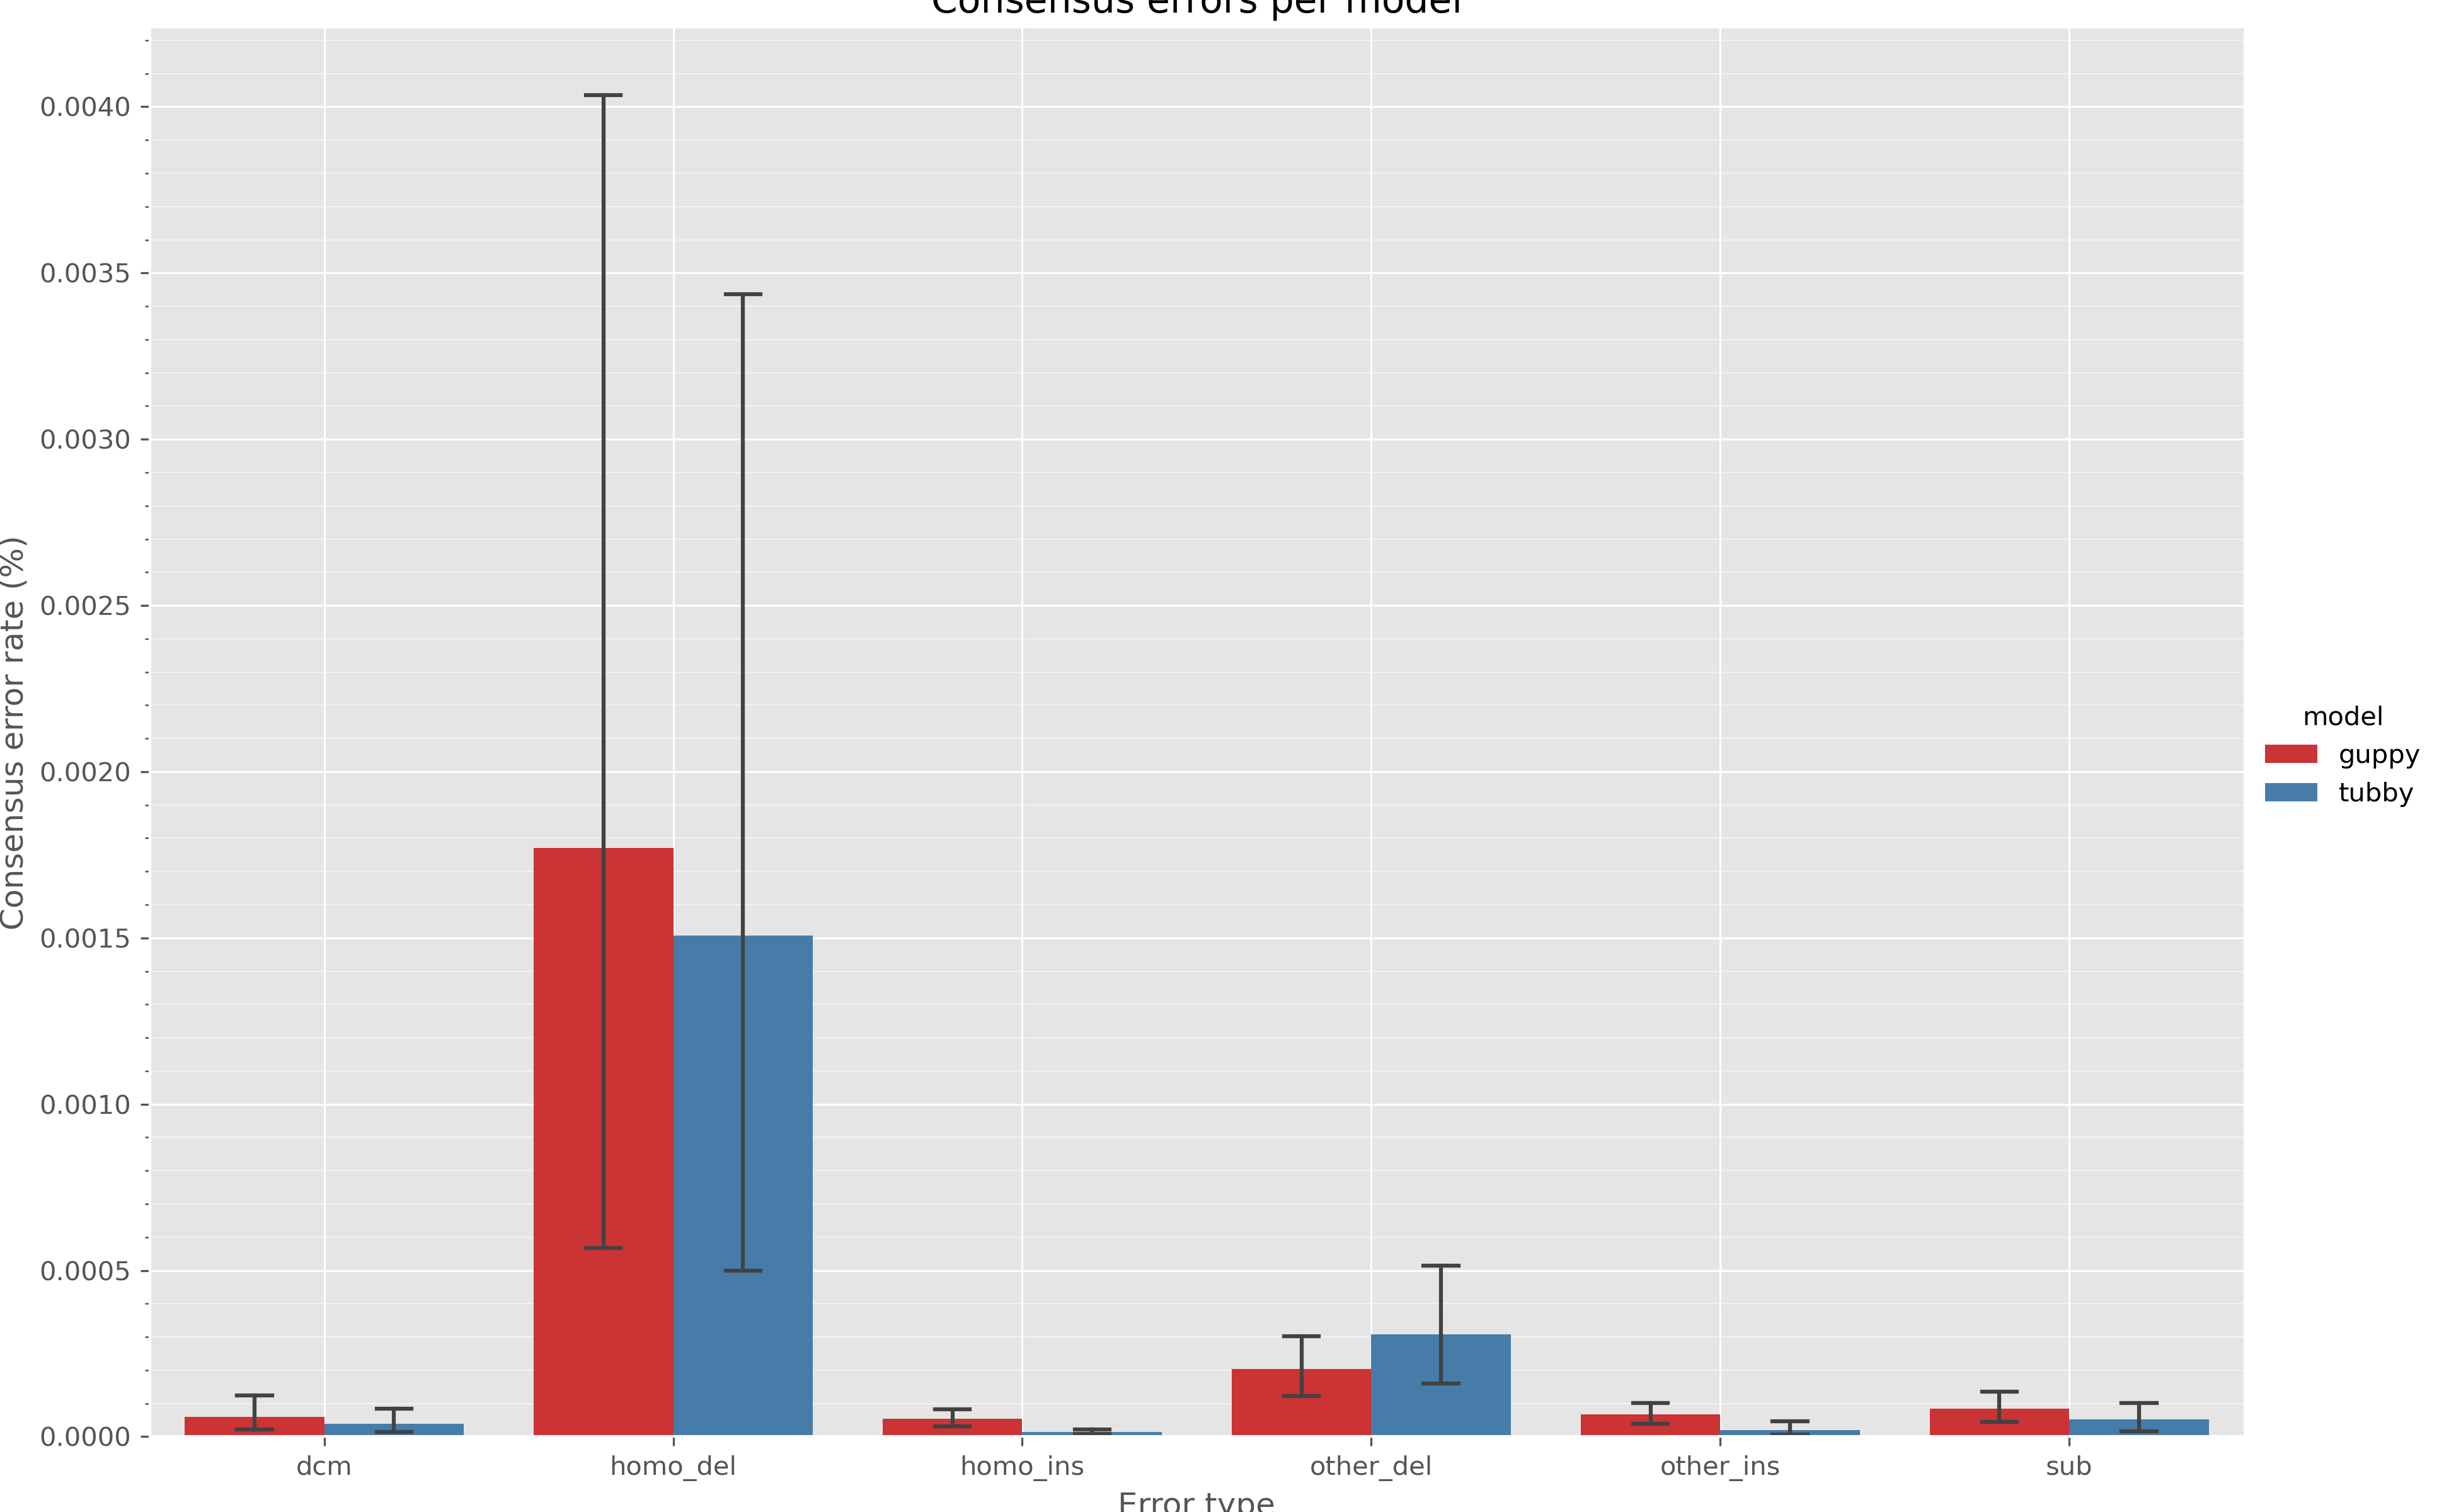
\includegraphics[width=1.0\textwidth]{Chapter4/Figs/consensus-error-types.png}
% \centering
% \caption{Error types in the \vrb{rebaler} assemblies produced from reads basecalled with tubby (blue) and \guppy{} (red). The consensus error rate is the percentage of the assembly these errors compose. The errors are per-assembly, so the confidence intervals represent variation in error types between samples/assemblies. dcm refers to Dcm-methylation motifs. homo\_ins/del are homopolymer insertions or deletions. sub is single-base substitutions.}
% \label{fig:error_types}
% \end{figure}

%%%%%%%%%%%%%%%%%%%%%%%%%%%%%%%%%%%%%%%%%%%%%%%%%%%%%%%%%%%%%%%%%%%%%%%%%%%%%%%%%
\section{Discussion}

%%%%%%%%%%%%%%%%%%%%%%%%%%%%%%%%%%%%%%%%%%%%%%%%%%%%%%%%%%%%%%%%%%%%%%%%%%%%%%%%%
\section{Conclusion}

%%%%%%%%%%%%%%%%%%%%%%%%%%%%%%%%%%%%%%%%%%%%%%%%%%%%%%%%%%%%%%%%%%%%%%%%%%%%%%%%%
\section{Future work}

%%%%%%%%%%%%%%%%%%%%%%%%%%%%%%%%%%%%%%%%%%%%%%%%%%%%%%%%%%%%%%%%%%%%%%%%%%%%%%%%%
\section{Availability of data and materials}